\documentclass[twoside]{book}

% Packages required by doxygen
\usepackage{calc}
\usepackage{doxygen}
\usepackage{graphicx}
\usepackage[utf8]{inputenc}
\usepackage{makeidx}
\usepackage{multicol}
\usepackage{multirow}
\usepackage{fixltx2e}
\PassOptionsToPackage{warn}{textcomp}
\usepackage{textcomp}
\usepackage[nointegrals]{wasysym}
\usepackage[table]{xcolor}

% Font selection
\usepackage[T1]{fontenc}
\usepackage{mathptmx}
\usepackage[scaled=.90]{helvet}
\usepackage{courier}
\usepackage{amssymb}
\usepackage{sectsty}
\renewcommand{\familydefault}{\sfdefault}
\allsectionsfont{%
  \fontseries{bc}\selectfont%
  \color{darkgray}%
}
\renewcommand{\DoxyLabelFont}{%
  \fontseries{bc}\selectfont%
  \color{darkgray}%
}
\newcommand{\+}{\discretionary{\mbox{\scriptsize$\hookleftarrow$}}{}{}}

% Page & text layout
\usepackage{geometry}
\geometry{%
  a4paper,%
  top=2.5cm,%
  bottom=2.5cm,%
  left=2.5cm,%
  right=2.5cm%
}
\tolerance=750
\hfuzz=15pt
\hbadness=750
\setlength{\emergencystretch}{15pt}
\setlength{\parindent}{0cm}
\setlength{\parskip}{0.2cm}
\makeatletter
\renewcommand{\paragraph}{%
  \@startsection{paragraph}{4}{0ex}{-1.0ex}{1.0ex}{%
    \normalfont\normalsize\bfseries\SS@parafont%
  }%
}
\renewcommand{\subparagraph}{%
  \@startsection{subparagraph}{5}{0ex}{-1.0ex}{1.0ex}{%
    \normalfont\normalsize\bfseries\SS@subparafont%
  }%
}
\makeatother

% Headers & footers
\usepackage{fancyhdr}
\pagestyle{fancyplain}
\fancyhead[LE]{\fancyplain{}{\bfseries\thepage}}
\fancyhead[CE]{\fancyplain{}{}}
\fancyhead[RE]{\fancyplain{}{\bfseries\leftmark}}
\fancyhead[LO]{\fancyplain{}{\bfseries\rightmark}}
\fancyhead[CO]{\fancyplain{}{}}
\fancyhead[RO]{\fancyplain{}{\bfseries\thepage}}
\fancyfoot[LE]{\fancyplain{}{}}
\fancyfoot[CE]{\fancyplain{}{}}
\fancyfoot[RE]{\fancyplain{}{\bfseries\scriptsize Generated on Sun Jun 1 2014 11\+:17\+:45 for Diff2\+D by Doxygen }}
\fancyfoot[LO]{\fancyplain{}{\bfseries\scriptsize Generated on Sun Jun 1 2014 11\+:17\+:45 for Diff2\+D by Doxygen }}
\fancyfoot[CO]{\fancyplain{}{}}
\fancyfoot[RO]{\fancyplain{}{}}
\renewcommand{\footrulewidth}{0.4pt}
\renewcommand{\chaptermark}[1]{%
  \markboth{#1}{}%
}
\renewcommand{\sectionmark}[1]{%
  \markright{\thesection\ #1}%
}

% Indices & bibliography
\usepackage{natbib}
\usepackage[titles]{tocloft}
\setcounter{tocdepth}{3}
\setcounter{secnumdepth}{5}
\makeindex

% Hyperlinks (required, but should be loaded last)
\usepackage{ifpdf}
\ifpdf
  \usepackage[pdftex,pagebackref=true]{hyperref}
\else
  \usepackage[ps2pdf,pagebackref=true]{hyperref}
\fi
\hypersetup{%
  colorlinks=true,%
  linkcolor=blue,%
  citecolor=blue,%
  unicode%
}

% Custom commands
\newcommand{\clearemptydoublepage}{%
  \newpage{\pagestyle{empty}\cleardoublepage}%
}


%===== C O N T E N T S =====

\begin{document}

% Titlepage & ToC
\hypersetup{pageanchor=false,
             bookmarks=true,
             bookmarksnumbered=true,
             pdfencoding=unicode
            }
\pagenumbering{roman}
\begin{titlepage}
\vspace*{7cm}
\begin{center}%
{\Large Diff2\+D }\\
\vspace*{1cm}
{\large Generated by Doxygen 1.8.7}\\
\vspace*{0.5cm}
{\small Sun Jun 1 2014 11:17:45}\\
\end{center}
\end{titlepage}
\clearemptydoublepage
\tableofcontents
\clearemptydoublepage
\pagenumbering{arabic}
\hypersetup{pageanchor=true}

%--- Begin generated contents ---
\chapter{Todo List}
\label{todo}
\hypertarget{todo}{}

\begin{DoxyRefList}
\item[\label{todo__todo000001}%
\hypertarget{todo__todo000001}{}%
Member \hyperlink{classProb_ad16bc67a7a966dd5b6ba38afbe85a860}{Prob\+:\+:solve\+\_\+serial} (std\+::string name, real cond, size\+\_\+t it\+\_\+outer, real R\+\_\+outer)]move this to class variable to avoid excess alloc! 
\end{DoxyRefList}
\chapter{Module Index}
\section{Modules}
Here is a list of all modules\+:\begin{DoxyCompactList}
\item \contentsline{section}{Core}{\pageref{group__group__core}}{}
\end{DoxyCompactList}

\chapter{Hierarchical Index}
\section{Class Hierarchy}
This inheritance list is sorted roughly, but not completely, alphabetically:\begin{DoxyCompactList}
\item \contentsline{section}{Conn}{\pageref{classConn}}{}
\item \contentsline{section}{EdgeError}{\pageref{structEdgeError}}{}
\item \contentsline{section}{Equation}{\pageref{classEquation}}{}
\item \contentsline{section}{Equation\_\-Prob}{\pageref{classEquation__Prob}}{}
\item \contentsline{section}{Index\_\-Lambda}{\pageref{structIndex__Lambda}}{}
\item \contentsline{section}{IS}{\pageref{structIS}}{}
\item \contentsline{section}{LocalCoor}{\pageref{classLocalCoor}}{}
\begin{DoxyCompactList}
\item \contentsline{section}{Face}{\pageref{classFace}}{}
\item \contentsline{section}{Patch}{\pageref{classPatch}}{}
\end{DoxyCompactList}
\item \contentsline{section}{NoIntersectError}{\pageref{structNoIntersectError}}{}
\item \contentsline{section}{Patch\_\-Group}{\pageref{classPatch__Group}}{}
\item \contentsline{section}{point\_\-not\_\-found}{\pageref{classpoint__not__found}}{}
\item \contentsline{section}{Prob}{\pageref{classProb}}{}
\item \contentsline{section}{Term}{\pageref{structTerm}}{}
\end{DoxyCompactList}

\chapter{Class Index}
\section{Class List}
Here are the classes, structs, unions and interfaces with brief descriptions:\begin{DoxyCompactList}
\item\contentsline{section}{\hyperlink{class____array}{\_\-\_\-array$<$ T, N $>$} }{\pageref{class____array}}{}
\item\contentsline{section}{\hyperlink{struct____multivec}{\_\-\_\-multivec$<$ D, U $>$} }{\pageref{struct____multivec}}{}
\item\contentsline{section}{\hyperlink{struct____multivec_3_011_00_01U_01_4}{\_\-\_\-multivec$<$ 1, U $>$} }{\pageref{struct____multivec_3_011_00_01U_01_4}}{}
\item\contentsline{section}{\hyperlink{classConn}{Conn} }{\pageref{classConn}}{}
\item\contentsline{section}{\hyperlink{structEdgeError}{EdgeError} }{\pageref{structEdgeError}}{}
\item\contentsline{section}{\hyperlink{classEquation}{Equation} }{\pageref{classEquation}}{}
\item\contentsline{section}{\hyperlink{classEquation__Prob}{Equation\_\-Prob} }{\pageref{classEquation__Prob}}{}
\item\contentsline{section}{\hyperlink{classFace}{Face} (Face )}{\pageref{classFace}}{}
\item\contentsline{section}{\hyperlink{structIndex__Lambda}{Index\_\-Lambda} }{\pageref{structIndex__Lambda}}{}
\item\contentsline{section}{\hyperlink{structInitializer__list}{Initializer\_\-list$<$ D, U $>$} }{\pageref{structInitializer__list}}{}
\item\contentsline{section}{\hyperlink{structInitializer__list_3_011_00_01U_01_4}{Initializer\_\-list$<$ 1, U $>$} }{\pageref{structInitializer__list_3_011_00_01U_01_4}}{}
\item\contentsline{section}{\hyperlink{structIS}{IS} }{\pageref{structIS}}{}
\item\contentsline{section}{\hyperlink{classLocalCoor}{LocalCoor} }{\pageref{classLocalCoor}}{}
\item\contentsline{section}{\hyperlink{structNoIntersectError}{NoIntersectError} }{\pageref{structNoIntersectError}}{}
\item\contentsline{section}{\hyperlink{classPatch}{Patch} }{\pageref{classPatch}}{}
\item\contentsline{section}{\hyperlink{classPatch__Group}{Patch\_\-Group} }{\pageref{classPatch__Group}}{}
\item\contentsline{section}{\hyperlink{classProb}{Prob} (Problem )}{\pageref{classProb}}{}
\item\contentsline{section}{\hyperlink{structTerm}{Term} }{\pageref{structTerm}}{}
\end{DoxyCompactList}

\chapter{File Index}
\section{File List}
Here is a list of all documented files with brief descriptions\+:\begin{DoxyCompactList}
\item\contentsline{section}{/nfs/stak/students/r/rymalc/\+Documents/\+Programming/\+C++/\+Diffusion2\+D/\+Debug/include/\+Diff2\+D/{\bfseries config.\+hpp} }{\pageref{config_8hpp}}{}
\item\contentsline{section}{/nfs/stak/students/r/rymalc/\+Documents/\+Programming/\+C++/\+Diffusion2\+D/include/\+Diff2\+D/{\bfseries boundary.\+hpp} }{\pageref{boundary_8hpp}}{}
\item\contentsline{section}{/nfs/stak/students/r/rymalc/\+Documents/\+Programming/\+C++/\+Diffusion2\+D/include/\+Diff2\+D/{\bfseries conn.\+hpp} }{\pageref{conn_8hpp}}{}
\item\contentsline{section}{/nfs/stak/students/r/rymalc/\+Documents/\+Programming/\+C++/\+Diffusion2\+D/include/\+Diff2\+D/{\bfseries decl.\+hpp} }{\pageref{decl_8hpp}}{}
\item\contentsline{section}{/nfs/stak/students/r/rymalc/\+Documents/\+Programming/\+C++/\+Diffusion2\+D/include/\+Diff2\+D/{\bfseries equation.\+hpp} }{\pageref{equation_8hpp}}{}
\item\contentsline{section}{/nfs/stak/students/r/rymalc/\+Documents/\+Programming/\+C++/\+Diffusion2\+D/include/\+Diff2\+D/{\bfseries face.\+hpp} }{\pageref{face_8hpp}}{}
\item\contentsline{section}{/nfs/stak/students/r/rymalc/\+Documents/\+Programming/\+C++/\+Diffusion2\+D/include/\+Diff2\+D/{\bfseries index\+\_\+lambda.\+hpp} }{\pageref{index__lambda_8hpp}}{}
\item\contentsline{section}{/nfs/stak/students/r/rymalc/\+Documents/\+Programming/\+C++/\+Diffusion2\+D/include/\+Diff2\+D/{\bfseries init.\+hpp} }{\pageref{init_8hpp}}{}
\item\contentsline{section}{/nfs/stak/students/r/rymalc/\+Documents/\+Programming/\+C++/\+Diffusion2\+D/include/\+Diff2\+D/{\bfseries log.\+hpp} }{\pageref{log_8hpp}}{}
\item\contentsline{section}{/nfs/stak/students/r/rymalc/\+Documents/\+Programming/\+C++/\+Diffusion2\+D/include/\+Diff2\+D/{\bfseries patch.\+hpp} }{\pageref{patch_8hpp}}{}
\item\contentsline{section}{/nfs/stak/students/r/rymalc/\+Documents/\+Programming/\+C++/\+Diffusion2\+D/include/\+Diff2\+D/{\bfseries patch\+\_\+group.\+hpp} }{\pageref{patch__group_8hpp}}{}
\item\contentsline{section}{/nfs/stak/students/r/rymalc/\+Documents/\+Programming/\+C++/\+Diffusion2\+D/include/\+Diff2\+D/{\bfseries point.\+hpp} }{\pageref{point_8hpp}}{}
\item\contentsline{section}{/nfs/stak/students/r/rymalc/\+Documents/\+Programming/\+C++/\+Diffusion2\+D/include/\+Diff2\+D/{\bfseries prob.\+hpp} }{\pageref{prob_8hpp}}{}
\item\contentsline{section}{/nfs/stak/students/r/rymalc/\+Documents/\+Programming/\+C++/\+Diffusion2\+D/include/\+Diff2\+D/{\bfseries stitch.\+hpp} }{\pageref{stitch_8hpp}}{}
\item\contentsline{section}{/nfs/stak/students/r/rymalc/\+Documents/\+Programming/\+C++/\+Diffusion2\+D/include/\+Diff2\+D/\hyperlink{types_8hpp}{types.\+hpp} }{\pageref{types_8hpp}}{}
\item\contentsline{section}{/nfs/stak/students/r/rymalc/\+Documents/\+Programming/\+C++/\+Diffusion2\+D/include/\+Diff2\+D/{\bfseries unit\+\_\+vec.\+hpp} }{\pageref{unit__vec_8hpp}}{}
\item\contentsline{section}{/nfs/stak/students/r/rymalc/\+Documents/\+Programming/\+C++/\+Diffusion2\+D/include/\+Diff2\+D/{\bfseries util.\+hpp} }{\pageref{util_8hpp}}{}
\end{DoxyCompactList}

\chapter{Module Documentation}
\hypertarget{group__group__core}{
\section{Core}
\label{group__group__core}\index{Core@{Core}}
}
\subsection*{Classes}
\begin{DoxyCompactItemize}
\item 
class \hyperlink{classFace}{Face}
\begin{DoxyCompactList}\small\item\em Face \item\end{DoxyCompactList}\item 
class \hyperlink{classProb}{Prob}
\begin{DoxyCompactList}\small\item\em Problem \item\end{DoxyCompactList}\end{DoxyCompactItemize}


\subsection{Detailed Description}
This group contains core objects 
\chapter{Class Documentation}
\hypertarget{structboundary}{\section{boundary Struct Reference}
\label{structboundary}\index{boundary@{boundary}}
}


Inheritance diagram for boundary\+:\nopagebreak
\begin{figure}[H]
\begin{center}
\leavevmode
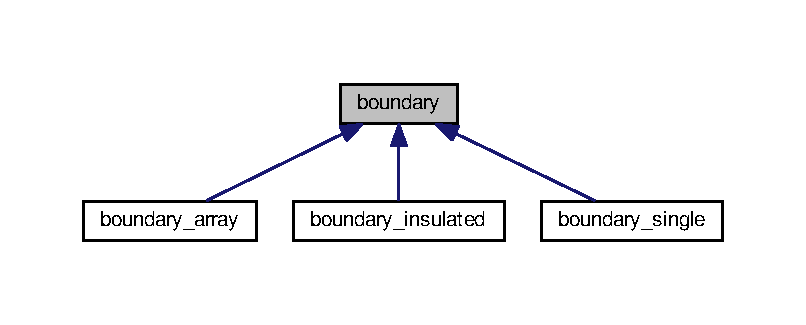
\includegraphics[width=350pt]{structboundary__inherit__graph}
\end{center}
\end{figure}
\subsection*{Public Member Functions}
\begin{DoxyCompactItemize}
\item 
\hypertarget{structboundary_a4a74d489d76ae54b9d7993b6f616976c}{virtual void {\bfseries eval} (std\+::shared\+\_\+ptr$<$ \hyperlink{classEquation}{Equation} $>$ const \&equ, std\+::vector$<$ int $>$ const \&ind, std\+::vector$<$ int $>$ const \&indn, unsigned int p)=0}\label{structboundary_a4a74d489d76ae54b9d7993b6f616976c}

\end{DoxyCompactItemize}


The documentation for this struct was generated from the following file\+:\begin{DoxyCompactItemize}
\item 
/nfs/stak/students/r/rymalc/\+Documents/\+Programming/\+C++/\+Diffusion2\+D/include/\+Diff2\+D/boundary.\+hpp\end{DoxyCompactItemize}

\hypertarget{structboundary__array}{\section{boundary\+\_\+array Struct Reference}
\label{structboundary__array}\index{boundary\+\_\+array@{boundary\+\_\+array}}
}


Inheritance diagram for boundary\+\_\+array\+:\nopagebreak
\begin{figure}[H]
\begin{center}
\leavevmode
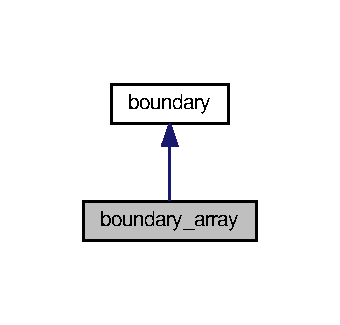
\includegraphics[width=163pt]{structboundary__array__inherit__graph}
\end{center}
\end{figure}


Collaboration diagram for boundary\+\_\+array\+:\nopagebreak
\begin{figure}[H]
\begin{center}
\leavevmode
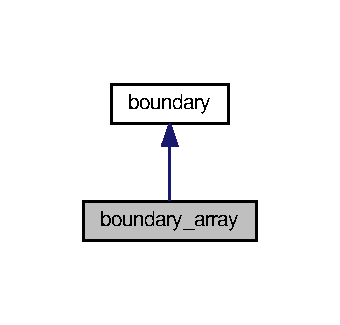
\includegraphics[width=163pt]{structboundary__array__coll__graph}
\end{center}
\end{figure}
\subsection*{Public Member Functions}
\begin{DoxyCompactItemize}
\item 
\hypertarget{structboundary__array_aa09696734c5db0908a66c59599751585}{{\bfseries boundary\+\_\+array} (array$<$ real, 1 $>$ v)}\label{structboundary__array_aa09696734c5db0908a66c59599751585}

\item 
\hypertarget{structboundary__array_ade5479ae68a0b88e4b16d572e671e436}{virtual void {\bfseries eval} (std\+::shared\+\_\+ptr$<$ \hyperlink{classEquation}{Equation} $>$ const \&equ, std\+::vector$<$ int $>$ const \&ind, std\+::vector$<$ int $>$ const \&indn, unsigned int p)}\label{structboundary__array_ade5479ae68a0b88e4b16d572e671e436}

\end{DoxyCompactItemize}
\subsection*{Public Attributes}
\begin{DoxyCompactItemize}
\item 
\hypertarget{structboundary__array_a803a5adfb6f046360e560cdac2830199}{array$<$ real, 1 $>$ {\bfseries v\+\_\+}}\label{structboundary__array_a803a5adfb6f046360e560cdac2830199}

\end{DoxyCompactItemize}


The documentation for this struct was generated from the following file\+:\begin{DoxyCompactItemize}
\item 
/nfs/stak/students/r/rymalc/\+Documents/\+Programming/\+C++/\+Diffusion2\+D/include/\+Diff2\+D/boundary.\+hpp\end{DoxyCompactItemize}

\hypertarget{structboundary__insulated}{\section{boundary\+\_\+insulated Struct Reference}
\label{structboundary__insulated}\index{boundary\+\_\+insulated@{boundary\+\_\+insulated}}
}


Inheritance diagram for boundary\+\_\+insulated\+:\nopagebreak
\begin{figure}[H]
\begin{center}
\leavevmode
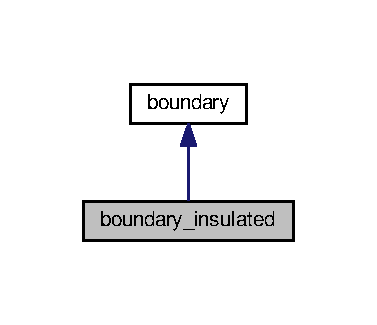
\includegraphics[width=181pt]{structboundary__insulated__inherit__graph}
\end{center}
\end{figure}


Collaboration diagram for boundary\+\_\+insulated\+:\nopagebreak
\begin{figure}[H]
\begin{center}
\leavevmode
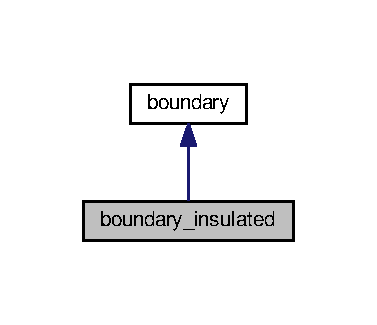
\includegraphics[width=181pt]{structboundary__insulated__coll__graph}
\end{center}
\end{figure}
\subsection*{Public Member Functions}
\begin{DoxyCompactItemize}
\item 
\hypertarget{structboundary__insulated_a738b5ea19e4dd105c312fdf33806ff5f}{virtual void {\bfseries eval} (std\+::shared\+\_\+ptr$<$ \hyperlink{classEquation}{Equation} $>$ const \&equ, std\+::vector$<$ int $>$ const \&ind, std\+::vector$<$ int $>$ const \&indn, unsigned int p)}\label{structboundary__insulated_a738b5ea19e4dd105c312fdf33806ff5f}

\end{DoxyCompactItemize}


The documentation for this struct was generated from the following file\+:\begin{DoxyCompactItemize}
\item 
/nfs/stak/students/r/rymalc/\+Documents/\+Programming/\+C++/\+Diffusion2\+D/include/\+Diff2\+D/boundary.\+hpp\end{DoxyCompactItemize}

\hypertarget{structboundary__single}{\section{boundary\+\_\+single Struct Reference}
\label{structboundary__single}\index{boundary\+\_\+single@{boundary\+\_\+single}}
}


Inheritance diagram for boundary\+\_\+single\+:\nopagebreak
\begin{figure}[H]
\begin{center}
\leavevmode
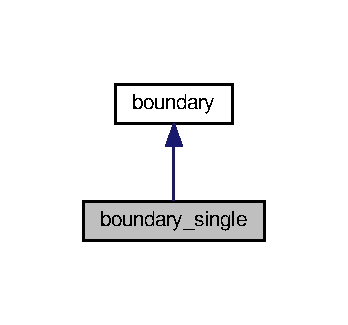
\includegraphics[width=167pt]{structboundary__single__inherit__graph}
\end{center}
\end{figure}


Collaboration diagram for boundary\+\_\+single\+:\nopagebreak
\begin{figure}[H]
\begin{center}
\leavevmode
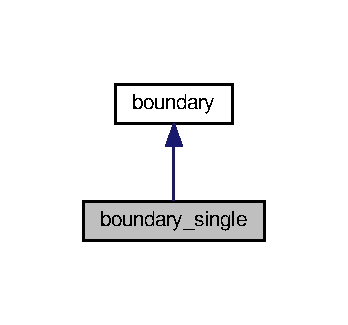
\includegraphics[width=167pt]{structboundary__single__coll__graph}
\end{center}
\end{figure}
\subsection*{Public Member Functions}
\begin{DoxyCompactItemize}
\item 
\hypertarget{structboundary__single_a794dda44938818af0e3f015b979a3d2f}{{\bfseries boundary\+\_\+single} (real v)}\label{structboundary__single_a794dda44938818af0e3f015b979a3d2f}

\item 
\hypertarget{structboundary__single_ad348670e49f4b8ab96cc35bce428a3f7}{virtual void {\bfseries eval} (std\+::shared\+\_\+ptr$<$ \hyperlink{classEquation}{Equation} $>$ const \&equ, std\+::vector$<$ int $>$ const \&ind, std\+::vector$<$ int $>$ const \&indn, unsigned int p)}\label{structboundary__single_ad348670e49f4b8ab96cc35bce428a3f7}

\end{DoxyCompactItemize}
\subsection*{Public Attributes}
\begin{DoxyCompactItemize}
\item 
\hypertarget{structboundary__single_a3aef38455e276f44418ae1c34803cce1}{real {\bfseries v\+\_\+}}\label{structboundary__single_a3aef38455e276f44418ae1c34803cce1}

\end{DoxyCompactItemize}


The documentation for this struct was generated from the following file\+:\begin{DoxyCompactItemize}
\item 
/nfs/stak/students/r/rymalc/\+Documents/\+Programming/\+C++/\+Diffusion2\+D/include/\+Diff2\+D/boundary.\+hpp\end{DoxyCompactItemize}

\hypertarget{classConn}{
\section{Conn Class Reference}
\label{classConn}\index{Conn@{Conn}}
}
Collaboration diagram for Conn:\nopagebreak
\begin{figure}[H]
\begin{center}
\leavevmode
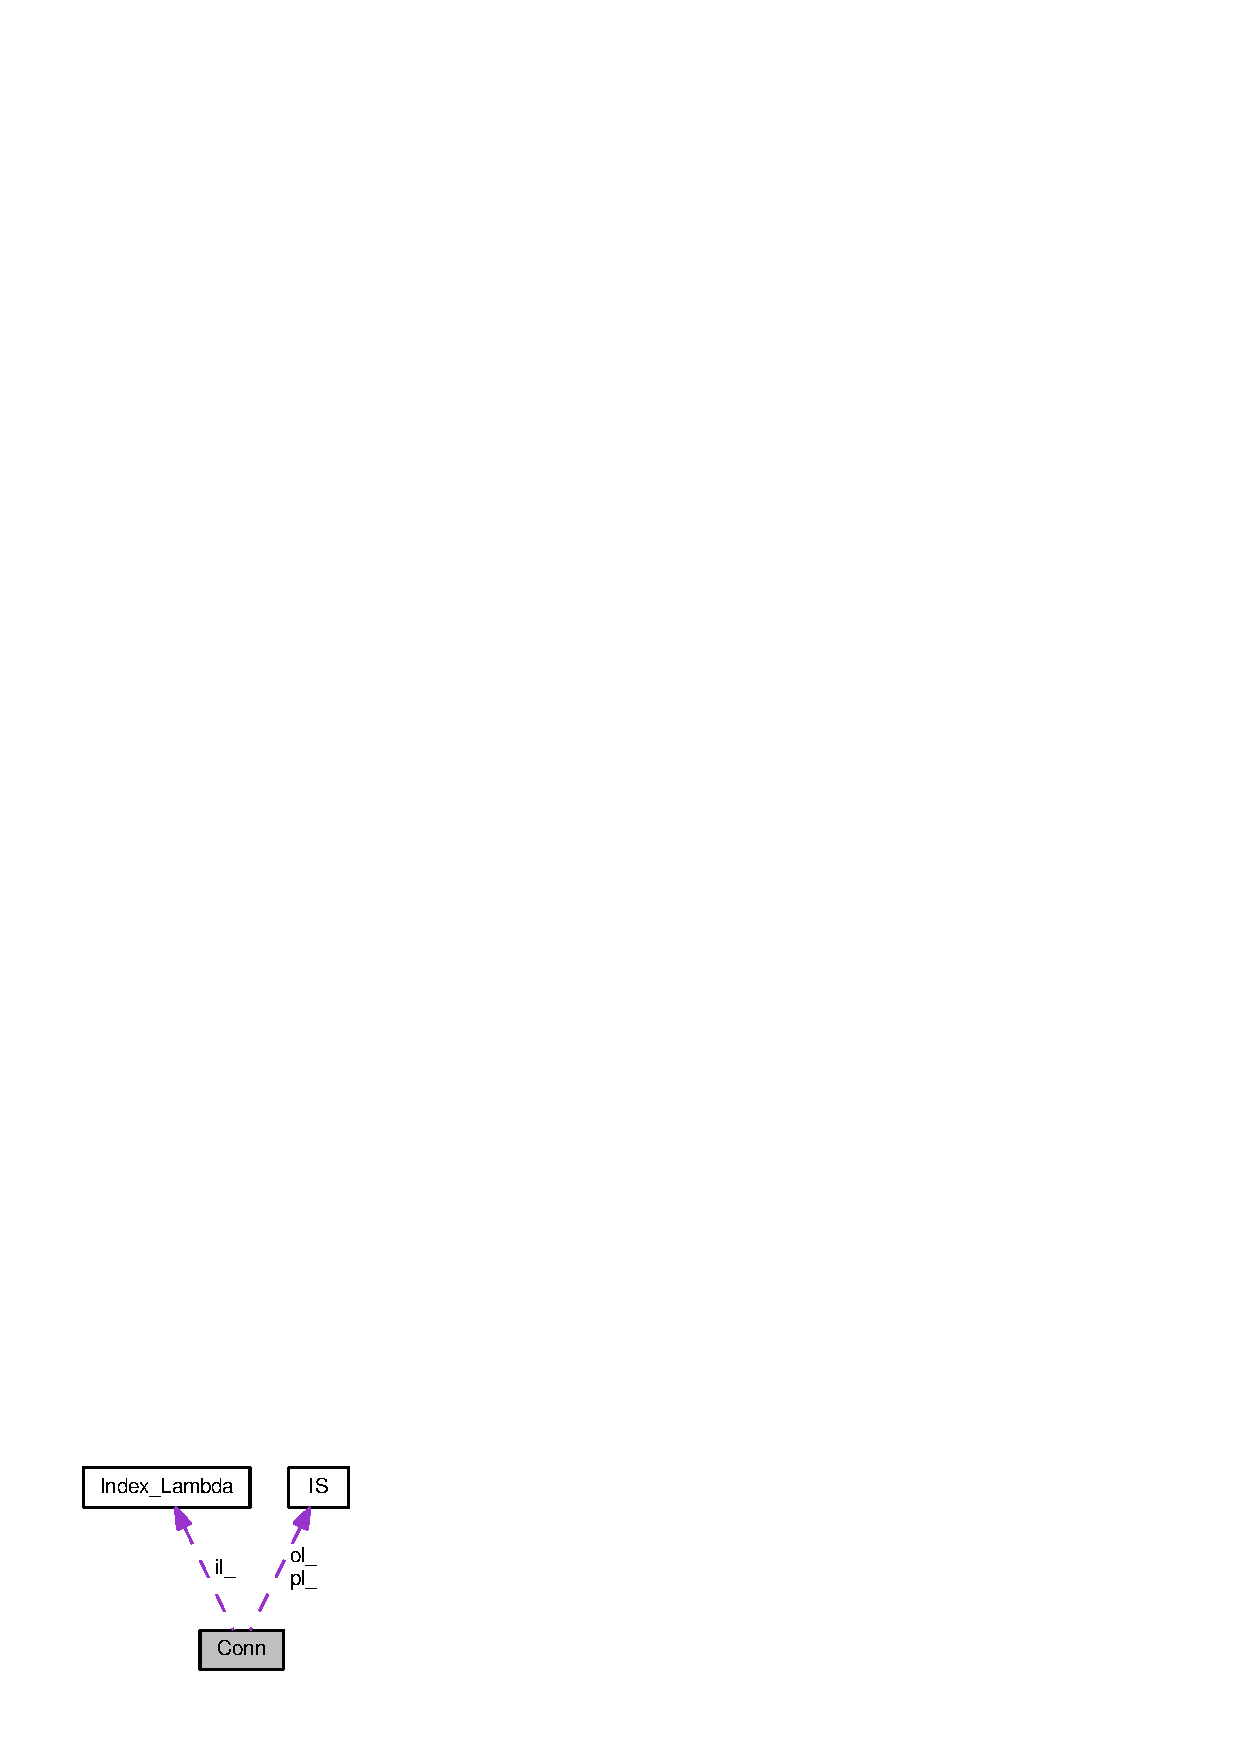
\includegraphics[width=172pt]{classConn__coll__graph}
\end{center}
\end{figure}
\subsection*{Public Member Functions}
\begin{DoxyCompactItemize}
\item 
\hypertarget{classConn_ab0ba4fbd67bc99991f2110c3ca80ca3d}{
{\bfseries Conn} (Face\_\-s face, void $\ast$conns)}
\label{classConn_ab0ba4fbd67bc99991f2110c3ca80ca3d}

\item 
\hypertarget{classConn_af3776731e374e856bb5eac3faea03ae3}{
void {\bfseries refresh} ()}
\label{classConn_af3776731e374e856bb5eac3faea03ae3}

\item 
\hypertarget{classConn_add96cc92a7575634f44220cb6e2e2421}{
void {\bfseries printinfo} ()}
\label{classConn_add96cc92a7575634f44220cb6e2e2421}

\item 
\hypertarget{classConn_ace36b6085ceadcfa9654b5950e7719c0}{
void {\bfseries send} (std::string name, array$<$ real, 1 $>$ v)}
\label{classConn_ace36b6085ceadcfa9654b5950e7719c0}

\item 
\hypertarget{classConn_a5f149a3217d7cf6227b48571638cadf8}{
array$<$ real, 1 $>$ {\bfseries recv} (std::string name)}
\label{classConn_a5f149a3217d7cf6227b48571638cadf8}

\end{DoxyCompactItemize}
\subsection*{Public Attributes}
\begin{DoxyCompactItemize}
\item 
\hypertarget{classConn_a61c9d519b93b91a14b4cc47a8cb8980b}{
\hyperlink{structIS}{IS} {\bfseries pl\_\-}}
\label{classConn_a61c9d519b93b91a14b4cc47a8cb8980b}

\item 
\hypertarget{classConn_a949773005bd6449b09e355e8f78dee47}{
\hyperlink{structIS}{IS} {\bfseries ol\_\-}}
\label{classConn_a949773005bd6449b09e355e8f78dee47}

\item 
\hypertarget{classConn_a8550bde616100c5f9cc23bc7ae267a18}{
int {\bfseries PG\_\-}}
\label{classConn_a8550bde616100c5f9cc23bc7ae267a18}

\item 
\hypertarget{classConn_a659caee9d9a125f24d7eb054ca2e5879}{
\hyperlink{structIndex__Lambda}{Index\_\-Lambda} {\bfseries il\_\-}}
\label{classConn_a659caee9d9a125f24d7eb054ca2e5879}

\item 
\hypertarget{classConn_a893abc608e559f12c5368edbd6da7b54}{
Face\_\-s {\bfseries face\_\-}}
\label{classConn_a893abc608e559f12c5368edbd6da7b54}

\item 
\hypertarget{classConn_a7578b2f58e208173f45436d7261271a0}{
Conn\_\-s {\bfseries twin\_\-}}
\label{classConn_a7578b2f58e208173f45436d7261271a0}

\item 
\hypertarget{classConn_ac571dea0fa3d37ed022872da32ad6c33}{
void $\ast$ {\bfseries conns\_\-}}
\label{classConn_ac571dea0fa3d37ed022872da32ad6c33}

\item 
\hypertarget{classConn_aae3bc6691f2e065bf44e8f1a2cd4e31f}{
bool {\bfseries parallel\_\-}}
\label{classConn_aae3bc6691f2e065bf44e8f1a2cd4e31f}

\item 
\hypertarget{classConn_a425d7d5713a82acbfa9a69adcc0c1c25}{
std::map$<$ std::string, array$<$ real, 1 $>$ $>$ {\bfseries equs\_\-}}
\label{classConn_a425d7d5713a82acbfa9a69adcc0c1c25}

\end{DoxyCompactItemize}


The documentation for this class was generated from the following files:\begin{DoxyCompactItemize}
\item 
/nfs/stak/students/r/rymalc/Documents/Programming/C++/Diffusion2D/include/Diff2D/conn.hpp\item 
/nfs/stak/students/r/rymalc/Documents/Programming/C++/Diffusion2D/src/Diff2D/conn.cpp\end{DoxyCompactItemize}

\hypertarget{structEdgeError}{\section{Edge\+Error Struct Reference}
\label{structEdgeError}\index{Edge\+Error@{Edge\+Error}}
}


Inheritance diagram for Edge\+Error\+:\nopagebreak
\begin{figure}[H]
\begin{center}
\leavevmode
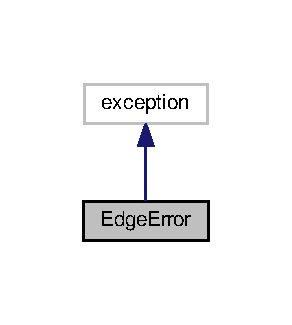
\includegraphics[width=140pt]{structEdgeError__inherit__graph}
\end{center}
\end{figure}


Collaboration diagram for Edge\+Error\+:\nopagebreak
\begin{figure}[H]
\begin{center}
\leavevmode
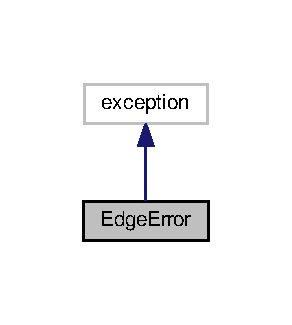
\includegraphics[width=140pt]{structEdgeError__coll__graph}
\end{center}
\end{figure}
\subsection*{Public Member Functions}
\begin{DoxyCompactItemize}
\item 
\hypertarget{structEdgeError_a92ca9588f65b2b4d17139ff80eb29ab3}{{\bfseries Edge\+Error} (bool rev)}\label{structEdgeError_a92ca9588f65b2b4d17139ff80eb29ab3}

\end{DoxyCompactItemize}
\subsection*{Public Attributes}
\begin{DoxyCompactItemize}
\item 
\hypertarget{structEdgeError_a704a81b20878f5b534df310ea179ae02}{bool {\bfseries rev\+\_\+}}\label{structEdgeError_a704a81b20878f5b534df310ea179ae02}

\end{DoxyCompactItemize}


The documentation for this struct was generated from the following file\+:\begin{DoxyCompactItemize}
\item 
/nfs/stak/students/r/rymalc/\+Documents/\+Programming/\+C++/\+Diffusion2\+D/include/\+Diff2\+D/util.\+hpp\end{DoxyCompactItemize}

\hypertarget{classEquation}{
\section{Equation Class Reference}
\label{classEquation}\index{Equation@{Equation}}
}
\subsection*{Public Types}
\begin{DoxyCompactItemize}
\item 
enum \{ {\bfseries ONLY\_\-PARALLEL\_\-FACES} =  1 $<$$<$ 0
 \}
\end{DoxyCompactItemize}
\subsection*{Public Member Functions}
\begin{DoxyCompactItemize}
\item 
\hypertarget{classEquation_aa828f4c9f7a849e9ae29f2c9491863d6}{
{\bfseries Equation} (std::string name, Face\_\-s face, Equation\_\-Prob\_\-s equ\_\-prob)}
\label{classEquation_aa828f4c9f7a849e9ae29f2c9491863d6}

\item 
\hypertarget{classEquation_acda03fc82a1a28ab32f127754bf37aea}{
array$<$ real, 3 $>$ {\bfseries grad} ()}
\label{classEquation_acda03fc82a1a28ab32f127754bf37aea}

\item 
\hypertarget{classEquation_ab67fb5e35d95e74756aed668b072c03f}{
real {\bfseries grad\_\-mag} ()}
\label{classEquation_ab67fb5e35d95e74756aed668b072c03f}

\item 
\hypertarget{classEquation_a629f1ff3c54e7fcfe597c20ab49c773b}{
real {\bfseries min} ()}
\label{classEquation_a629f1ff3c54e7fcfe597c20ab49c773b}

\item 
\hypertarget{classEquation_a1e95e7d54591e5dc5c68ccca547101c5}{
real {\bfseries max} ()}
\label{classEquation_a1e95e7d54591e5dc5c68ccca547101c5}

\item 
\hypertarget{classEquation_a3a22bc1a6dd067b6feaf6fc6281a5c1f}{
real {\bfseries grad\_\-min} ()}
\label{classEquation_a3a22bc1a6dd067b6feaf6fc6281a5c1f}

\item 
\hypertarget{classEquation_ae2b284533eda56200c9122846623eb45}{
real {\bfseries grad\_\-max} ()}
\label{classEquation_ae2b284533eda56200c9122846623eb45}

\item 
\hypertarget{classEquation_ae0198edcc6a9a44ed7d88d8279f91cee}{
real {\bfseries mean} ()}
\label{classEquation_ae0198edcc6a9a44ed7d88d8279f91cee}

\item 
\hypertarget{classEquation_a780d64d5a94161a5cf71d0d08a6ffe5b}{
real {\bfseries point} (real pt\mbox{[}2\mbox{]})}
\label{classEquation_a780d64d5a94161a5cf71d0d08a6ffe5b}

\end{DoxyCompactItemize}
\subsection*{Public Attributes}
\begin{DoxyCompactItemize}
\item 
\hypertarget{classEquation_a2bbb65c98ebf1345231370e93b504037}{
std::string {\bfseries name\_\-}}
\label{classEquation_a2bbb65c98ebf1345231370e93b504037}

\item 
\hypertarget{classEquation_a9eeeceed0d8130fd30fb2e65f3b15f3f}{
Face\_\-s {\bfseries face\_\-}}
\label{classEquation_a9eeeceed0d8130fd30fb2e65f3b15f3f}

\item 
\hypertarget{classEquation_a1ece93bf1c58eb22001327da69ab73fc}{
Equation\_\-Prob\_\-s {\bfseries equ\_\-prob\_\-}}
\label{classEquation_a1ece93bf1c58eb22001327da69ab73fc}

\item 
\hypertarget{classEquation_ac7f793f3b1e3694b719d91d884460880}{
array$<$ real, 2 $>$ {\bfseries s\_\-}}
\label{classEquation_ac7f793f3b1e3694b719d91d884460880}

\item 
\hypertarget{classEquation_aa48c28c116aec278f7713a414dec6196}{
array$<$ real, 2 $>$ {\bfseries v\_\-}}
\label{classEquation_aa48c28c116aec278f7713a414dec6196}

\item 
\hypertarget{classEquation_a1820f1ab792e83981456fce5dda492b9}{
unsigned int {\bfseries flag\_\-}}
\label{classEquation_a1820f1ab792e83981456fce5dda492b9}

\item 
\hypertarget{classEquation_ab4039b291316d3a42c43330e868b4f50}{
multivec$<$ 2, array$<$ real, 1 $>$ $>$ {\bfseries v\_\-bou\_\-}}
\label{classEquation_ab4039b291316d3a42c43330e868b4f50}

\end{DoxyCompactItemize}


The documentation for this class was generated from the following files:\begin{DoxyCompactItemize}
\item 
/nfs/stak/students/r/rymalc/Documents/Programming/C++/Diffusion2D/include/Diff2D/equation.hpp\item 
/nfs/stak/students/r/rymalc/Documents/Programming/C++/Diffusion2D/src/Diff2D/equation.cpp\end{DoxyCompactItemize}

\hypertarget{classEquation__Prob}{
\section{Equation\_\-Prob Class Reference}
\label{classEquation__Prob}\index{Equation\_\-Prob@{Equation\_\-Prob}}
}
\subsection*{Public Member Functions}
\begin{DoxyCompactItemize}
\item 
\hypertarget{classEquation__Prob_a8eda60c6fe1e289ac5384cdf530cb47b}{
{\bfseries Equation\_\-Prob} (Prob\_\-s prob, std::string name, real k, real alpha, real alpha\_\-source)}
\label{classEquation__Prob_a8eda60c6fe1e289ac5384cdf530cb47b}

\end{DoxyCompactItemize}
\subsection*{Public Attributes}
\begin{DoxyCompactItemize}
\item 
\hypertarget{classEquation__Prob_a8761e4cfb7c9c934d1827a91625d7643}{
Prob\_\-s {\bfseries prob\_\-}}
\label{classEquation__Prob_a8761e4cfb7c9c934d1827a91625d7643}

\item 
\hypertarget{classEquation__Prob_af9c78d17a5b69f44175e95cef57c05d3}{
std::string {\bfseries name\_\-}}
\label{classEquation__Prob_af9c78d17a5b69f44175e95cef57c05d3}

\item 
\hypertarget{classEquation__Prob_add8db541a0ff4a402b95e2a70a3ad7a8}{
real {\bfseries k\_\-}}
\label{classEquation__Prob_add8db541a0ff4a402b95e2a70a3ad7a8}

\item 
\hypertarget{classEquation__Prob_ab8c2b9f46d6d9393c6556d0e734aae61}{
real {\bfseries alpha\_\-}}
\label{classEquation__Prob_ab8c2b9f46d6d9393c6556d0e734aae61}

\item 
\hypertarget{classEquation__Prob_aeb3f0d6aa0ffbbd16bc0866f177ec13e}{
real {\bfseries alpha\_\-source\_\-}}
\label{classEquation__Prob_aeb3f0d6aa0ffbbd16bc0866f177ec13e}

\end{DoxyCompactItemize}


The documentation for this class was generated from the following files:\begin{DoxyCompactItemize}
\item 
/nfs/stak/students/r/rymalc/Documents/Programming/C++/Diffusion2D/include/Diff2D/equation.hpp\item 
/nfs/stak/students/r/rymalc/Documents/Programming/C++/Diffusion2D/src/Diff2D/equation.cpp\end{DoxyCompactItemize}

\hypertarget{classFace}{
\section{Face Class Reference}
\label{classFace}\index{Face@{Face}}
}


Face  


{\ttfamily \#include $<$face.hpp$>$}Inheritance diagram for Face:\nopagebreak
\begin{figure}[H]
\begin{center}
\leavevmode
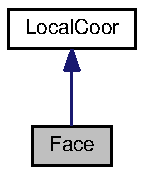
\includegraphics[width=105pt]{classFace__inherit__graph}
\end{center}
\end{figure}
Collaboration diagram for Face:\nopagebreak
\begin{figure}[H]
\begin{center}
\leavevmode
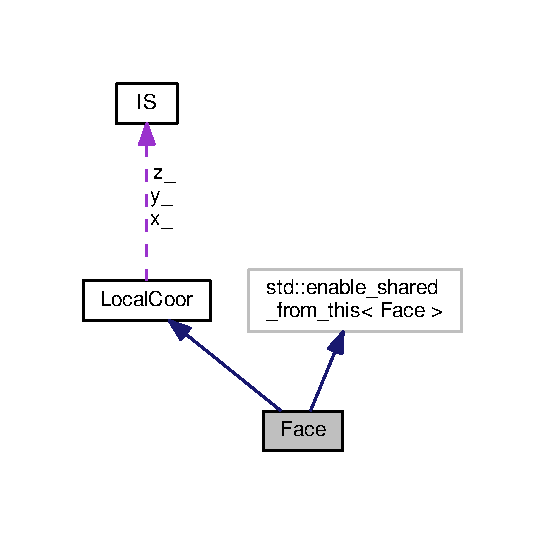
\includegraphics[width=400pt]{classFace__coll__graph}
\end{center}
\end{figure}
\subsection*{Public Member Functions}
\begin{DoxyCompactItemize}
\item 
\hypertarget{classFace_a66d5955aa6386be0fd482a5ac1174229}{
{\bfseries Face} (Patch\_\-s patch, int normal, array$<$ real, 2 $>$ const \&ext, real pos\_\-z, array$<$ size\_\-t, 1 $>$ n)}
\label{classFace_a66d5955aa6386be0fd482a5ac1174229}

\item 
\hypertarget{classFace_a5e444cef6d1f3fb3b7d64a4799f59eb9}{
Equation\_\-s {\bfseries create\_\-equ} (std::string name, Equation\_\-Prob\_\-s equ\_\-prob)}
\label{classFace_a5e444cef6d1f3fb3b7d64a4799f59eb9}

\item 
\hypertarget{classFace_a7ebc4163752a05d82e184a3a4c8671b3}{
int {\bfseries get\_\-loc\_\-pos\_\-par\_\-index} (Face\_\-s nbr)}
\label{classFace_a7ebc4163752a05d82e184a3a4c8671b3}

\item 
\hypertarget{classFace_aed5980668f26bc29338dfa11b32919f5}{
real {\bfseries x} (int i)}
\label{classFace_aed5980668f26bc29338dfa11b32919f5}

\item 
\hypertarget{classFace_a9a4d892bf5e8782c898e15aa5a989806}{
real {\bfseries y} (int j)}
\label{classFace_a9a4d892bf5e8782c898e15aa5a989806}

\item 
\hypertarget{classFace_a2d20ebd0d99063967bb26657abebbcbe}{
real {\bfseries area} ()}
\label{classFace_a2d20ebd0d99063967bb26657abebbcbe}

\item 
\hypertarget{classFace_a06eb55371bc742e523a9eb94a573209d}{
int {\bfseries nbr\_\-to\_\-loc} (Face\_\-s nbr)}
\label{classFace_a06eb55371bc742e523a9eb94a573209d}

\item 
\hypertarget{classFace_a60baec409a104a88e6622efa2f80122c}{
Conn\_\-s {\bfseries loc\_\-to\_\-conn} (int V)}
\label{classFace_a60baec409a104a88e6622efa2f80122c}

\item 
\hypertarget{classFace_a9a5eb93863dc767848261afa813ca039}{
\hyperlink{structIndex__Lambda}{Index\_\-Lambda} {\bfseries index\_\-lambda} (Face\_\-s nbr)}
\label{classFace_a9a5eb93863dc767848261afa813ca039}

\item 
\hypertarget{classFace_afdbbc9947c0d7cd84b427bd7b503b15b}{
void {\bfseries send\_\-array} (Equation\_\-s equ, Conn\_\-s conn)}
\label{classFace_afdbbc9947c0d7cd84b427bd7b503b15b}

\item 
\hypertarget{classFace_a57bdfcf1ebf5e208b611f98b7ddeca00}{
void {\bfseries recv\_\-array} (Equation\_\-s equ, Conn\_\-s conn)}
\label{classFace_a57bdfcf1ebf5e208b611f98b7ddeca00}

\item 
\hypertarget{classFace_aa827a7d26d1b90507bb4252830b3ecf5}{
\hyperlink{structTerm}{Term} {\bfseries term} (Equation\_\-s equ, std::vector$<$ int $>$ ind, int v, int sv, real To)}
\label{classFace_aa827a7d26d1b90507bb4252830b3ecf5}

\item 
\hypertarget{classFace_aba0d776b0f0e7cceee8729825347b5cc}{
void {\bfseries step\_\-pre\_\-cell} (Equation\_\-s equ, std::vector$<$ int $>$ ind, int V)}
\label{classFace_aba0d776b0f0e7cceee8729825347b5cc}

\item 
\hypertarget{classFace_a2bafbcce9f57fd3bdefd9f23a62c853d}{
void {\bfseries step\_\-pre\_\-cell\_\-open\_\-bou} (Equation\_\-s equ, std::vector$<$ int $>$ ind, int V)}
\label{classFace_a2bafbcce9f57fd3bdefd9f23a62c853d}

\item 
\hypertarget{classFace_a8af2298846b8a666332f00de91796844}{
void {\bfseries step\_\-pre} (Equation\_\-s equ)}
\label{classFace_a8af2298846b8a666332f00de91796844}

\item 
\hypertarget{classFace_a62a7d504c1e99dfc928b7e27b544893b}{
real {\bfseries step} (std::string equ\_\-name)}
\label{classFace_a62a7d504c1e99dfc928b7e27b544893b}

\item 
\hypertarget{classFace_a781b3843f33507116afa741579317e83}{
void {\bfseries send} (std::string equ\_\-name)}
\label{classFace_a781b3843f33507116afa741579317e83}

\item 
\hypertarget{classFace_a4c67c45fa975e6fb3bc3d4ee0fa6a25f}{
void {\bfseries recv} (std::string equ\_\-name)}
\label{classFace_a4c67c45fa975e6fb3bc3d4ee0fa6a25f}

\item 
\hypertarget{classFace_a18aba75abf718dd35c17153220ad929b}{
grid\_\-tup {\bfseries grid} (std::string equ\_\-name)}
\label{classFace_a18aba75abf718dd35c17153220ad929b}

\end{DoxyCompactItemize}
\subsection*{Public Attributes}
\begin{DoxyCompactItemize}
\item 
\hypertarget{classFace_a2e53c055a4d8492b42995db563e1fc7a}{
Patch\_\-s {\bfseries patch\_\-}}
\label{classFace_a2e53c055a4d8492b42995db563e1fc7a}

\item 
\hypertarget{classFace_a0922668c4175d0274024a5869b310a63}{
array$<$ real, 2 $>$ {\bfseries ext\_\-}}
\label{classFace_a0922668c4175d0274024a5869b310a63}

\item 
\hypertarget{classFace_ac831a8581fa641c54f4adb6e6b3dfe71}{
std::vector$<$ std::vector$<$ Conn\_\-s $>$ $>$ {\bfseries conns\_\-}}
\label{classFace_ac831a8581fa641c54f4adb6e6b3dfe71}

\item 
\hypertarget{classFace_a639f6d684b3a55d69528b5b6f5976937}{
real {\bfseries pos\_\-z\_\-}}
\label{classFace_a639f6d684b3a55d69528b5b6f5976937}

\item 
\hypertarget{classFace_af798b428f231a2f7fad13a386a5c4d7f}{
array$<$ size\_\-t, 1 $>$ {\bfseries n\_\-}}
\label{classFace_af798b428f231a2f7fad13a386a5c4d7f}

\item 
\hypertarget{classFace_a7d41239f934e8819874b5fb515d43380}{
array$<$ real, 3 $>$ {\bfseries d\_\-}}
\label{classFace_a7d41239f934e8819874b5fb515d43380}

\item 
\hypertarget{classFace_a75033fb2521fcb2c613782f831f42bb3}{
array$<$ real, 1 $>$ {\bfseries l\_\-}}
\label{classFace_a75033fb2521fcb2c613782f831f42bb3}

\item 
\hypertarget{classFace_a46b37a1eaba00ad44cf46b6da1391b30}{
std::map$<$ std::string, Equation\_\-s $>$ {\bfseries equs\_\-}}
\label{classFace_a46b37a1eaba00ad44cf46b6da1391b30}

\end{DoxyCompactItemize}


\subsection{Detailed Description}
Face 

The documentation for this class was generated from the following files:\begin{DoxyCompactItemize}
\item 
/nfs/stak/students/r/rymalc/Documents/Programming/C++/Diffusion2D/include/Diff2D/face.hpp\item 
/nfs/stak/students/r/rymalc/Documents/Programming/C++/Diffusion2D/src/Diff2D/face.cpp\end{DoxyCompactItemize}

\hypertarget{structIndex__Lambda}{\section{Index\+\_\+\+Lambda Struct Reference}
\label{structIndex__Lambda}\index{Index\+\_\+\+Lambda@{Index\+\_\+\+Lambda}}
}
\subsection*{Public Member Functions}
\begin{DoxyCompactItemize}
\item 
\hypertarget{structIndex__Lambda_af8225252f38290763a8aae14a0660a02}{int {\bfseries operator()} (int i, int p)}\label{structIndex__Lambda_af8225252f38290763a8aae14a0660a02}

\end{DoxyCompactItemize}
\subsection*{Public Attributes}
\begin{DoxyCompactItemize}
\item 
\hypertarget{structIndex__Lambda_acdf68b7c6f870f4eeb4ee9d8183e0c73}{int {\bfseries a} \mbox{[}2\mbox{]}}\label{structIndex__Lambda_acdf68b7c6f870f4eeb4ee9d8183e0c73}

\item 
\hypertarget{structIndex__Lambda_aaa095d0d1b30bc698d5a816ff0199951}{int {\bfseries b} \mbox{[}2\mbox{]}}\label{structIndex__Lambda_aaa095d0d1b30bc698d5a816ff0199951}

\item 
\hypertarget{structIndex__Lambda_a34e9306034a5059d37f4ab53d79ea5c7}{real {\bfseries d}}\label{structIndex__Lambda_a34e9306034a5059d37f4ab53d79ea5c7}

\end{DoxyCompactItemize}


The documentation for this struct was generated from the following file\+:\begin{DoxyCompactItemize}
\item 
/nfs/stak/students/r/rymalc/\+Documents/\+Programming/\+C++/\+Diffusion2\+D/include/\+Diff2\+D/index\+\_\+lambda.\+hpp\end{DoxyCompactItemize}

\hypertarget{structIS}{
\section{IS Struct Reference}
\label{structIS}\index{IS@{IS}}
}
\subsection*{Public Member Functions}
\begin{DoxyCompactItemize}
\item 
\hypertarget{structIS_aec66c50fd699031a1f617117c67eda11}{
\hyperlink{structIS}{IS} \& {\bfseries operator=} (\hyperlink{structIS}{IS} const \&is)}
\label{structIS_aec66c50fd699031a1f617117c67eda11}

\item 
\hypertarget{structIS_a2cb6d148c70406c11b9508be2cfddd7e}{
{\bfseries IS} (int ni, int ns)}
\label{structIS_a2cb6d148c70406c11b9508be2cfddd7e}

\item 
\hypertarget{structIS_a53883df04399eab305d240898e889271}{
{\bfseries IS} (int v)}
\label{structIS_a53883df04399eab305d240898e889271}

\item 
\hypertarget{structIS_ad474289c5f0f5f5b231cd2067547cc0f}{
int {\bfseries v} ()}
\label{structIS_ad474289c5f0f5f5b231cd2067547cc0f}

\end{DoxyCompactItemize}
\subsection*{Public Attributes}
\begin{DoxyCompactItemize}
\item 
\hypertarget{structIS_ac0a890989ec0d04b8db157583b154c17}{
int {\bfseries i}}
\label{structIS_ac0a890989ec0d04b8db157583b154c17}

\item 
\hypertarget{structIS_a3a4dc37a5dc69fa81e33c5e7115dca71}{
int {\bfseries s}}
\label{structIS_a3a4dc37a5dc69fa81e33c5e7115dca71}

\end{DoxyCompactItemize}


The documentation for this struct was generated from the following file:\begin{DoxyCompactItemize}
\item 
/nfs/stak/students/r/rymalc/Documents/Programming/C++/Diffusion2D/include/Diff2D/unit\_\-vec.hpp\end{DoxyCompactItemize}

\hypertarget{classLocalCoor}{
\section{LocalCoor Class Reference}
\label{classLocalCoor}\index{LocalCoor@{LocalCoor}}
}
Inheritance diagram for LocalCoor:\nopagebreak
\begin{figure}[H]
\begin{center}
\leavevmode
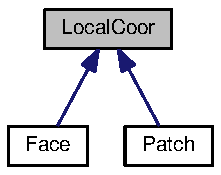
\includegraphics[width=142pt]{classLocalCoor__inherit__graph}
\end{center}
\end{figure}
Collaboration diagram for LocalCoor:\nopagebreak
\begin{figure}[H]
\begin{center}
\leavevmode
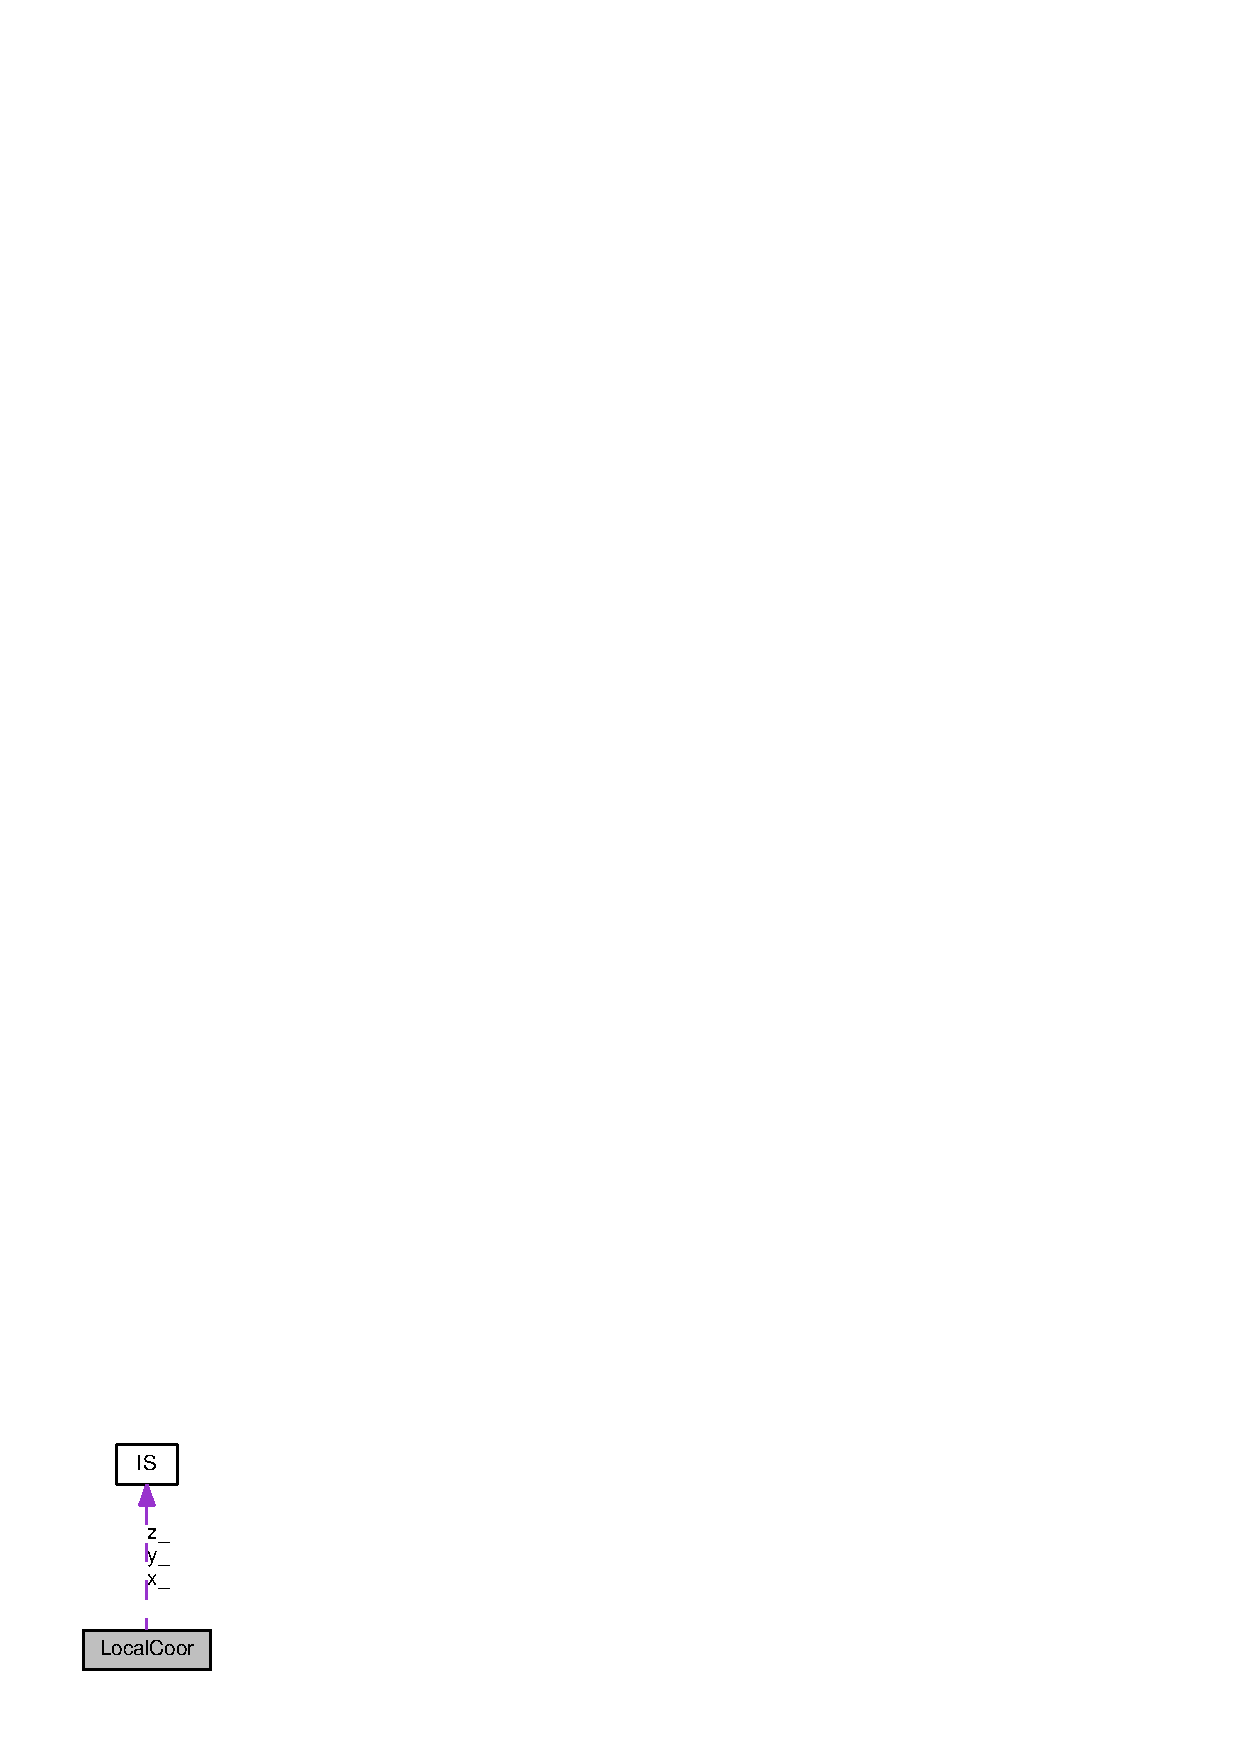
\includegraphics[width=105pt]{classLocalCoor__coll__graph}
\end{center}
\end{figure}
\subsection*{Public Member Functions}
\begin{DoxyCompactItemize}
\item 
\hypertarget{classLocalCoor_a00f6c0c9e48e46f15e1aaf36331fedeb}{
{\bfseries LocalCoor} (int Z)}
\label{classLocalCoor_a00f6c0c9e48e46f15e1aaf36331fedeb}

\item 
\hypertarget{classLocalCoor_ab96f489ba970f19b22e75f94bbec99c1}{
int {\bfseries glo\_\-to\_\-loc} (int G)}
\label{classLocalCoor_ab96f489ba970f19b22e75f94bbec99c1}

\item 
\hypertarget{classLocalCoor_ab5da8e4b3f6c32fbf6636aaa47e04adc}{
int {\bfseries loc\_\-to\_\-glo} (int L)}
\label{classLocalCoor_ab5da8e4b3f6c32fbf6636aaa47e04adc}

\end{DoxyCompactItemize}
\subsection*{Public Attributes}
\begin{DoxyCompactItemize}
\item 
\hypertarget{classLocalCoor_acd97c2eb7e3b994dbc58ae98ab785280}{
int {\bfseries Z\_\-}}
\label{classLocalCoor_acd97c2eb7e3b994dbc58ae98ab785280}

\item 
\hypertarget{classLocalCoor_a7d72e3489aaf1b6579f7a3e0f5b30e26}{
int {\bfseries X\_\-}}
\label{classLocalCoor_a7d72e3489aaf1b6579f7a3e0f5b30e26}

\item 
\hypertarget{classLocalCoor_a5ff6668d5d6898582ddfdc5eadce58ff}{
int {\bfseries Y\_\-}}
\label{classLocalCoor_a5ff6668d5d6898582ddfdc5eadce58ff}

\item 
\hypertarget{classLocalCoor_a2c0e974fc45c597f893b20a0c2f6869c}{
\hyperlink{structIS}{IS} {\bfseries x\_\-}}
\label{classLocalCoor_a2c0e974fc45c597f893b20a0c2f6869c}

\item 
\hypertarget{classLocalCoor_a58678d9cfb17db349a9d7fd70a2d5150}{
\hyperlink{structIS}{IS} {\bfseries y\_\-}}
\label{classLocalCoor_a58678d9cfb17db349a9d7fd70a2d5150}

\item 
\hypertarget{classLocalCoor_acdd6d24c450a43fd755f2e43d16d9991}{
\hyperlink{structIS}{IS} {\bfseries z\_\-}}
\label{classLocalCoor_acdd6d24c450a43fd755f2e43d16d9991}

\end{DoxyCompactItemize}


The documentation for this class was generated from the following files:\begin{DoxyCompactItemize}
\item 
/nfs/stak/students/r/rymalc/Documents/Programming/C++/Diffusion2D/include/Diff2D/unit\_\-vec.hpp\item 
/nfs/stak/students/r/rymalc/Documents/Programming/C++/Diffusion2D/src/Diff2D/LocalCoor.cpp\end{DoxyCompactItemize}

\hypertarget{structNoIntersectError}{
\section{NoIntersectError Struct Reference}
\label{structNoIntersectError}\index{NoIntersectError@{NoIntersectError}}
}


The documentation for this struct was generated from the following file:\begin{DoxyCompactItemize}
\item 
/nfs/stak/students/r/rymalc/Documents/Programming/C++/Diffusion2D/src/Diff2D/util.cpp\end{DoxyCompactItemize}

\hypertarget{classPatch}{\section{Patch Class Reference}
\label{classPatch}\index{Patch@{Patch}}
}


Inheritance diagram for Patch\+:\nopagebreak
\begin{figure}[H]
\begin{center}
\leavevmode
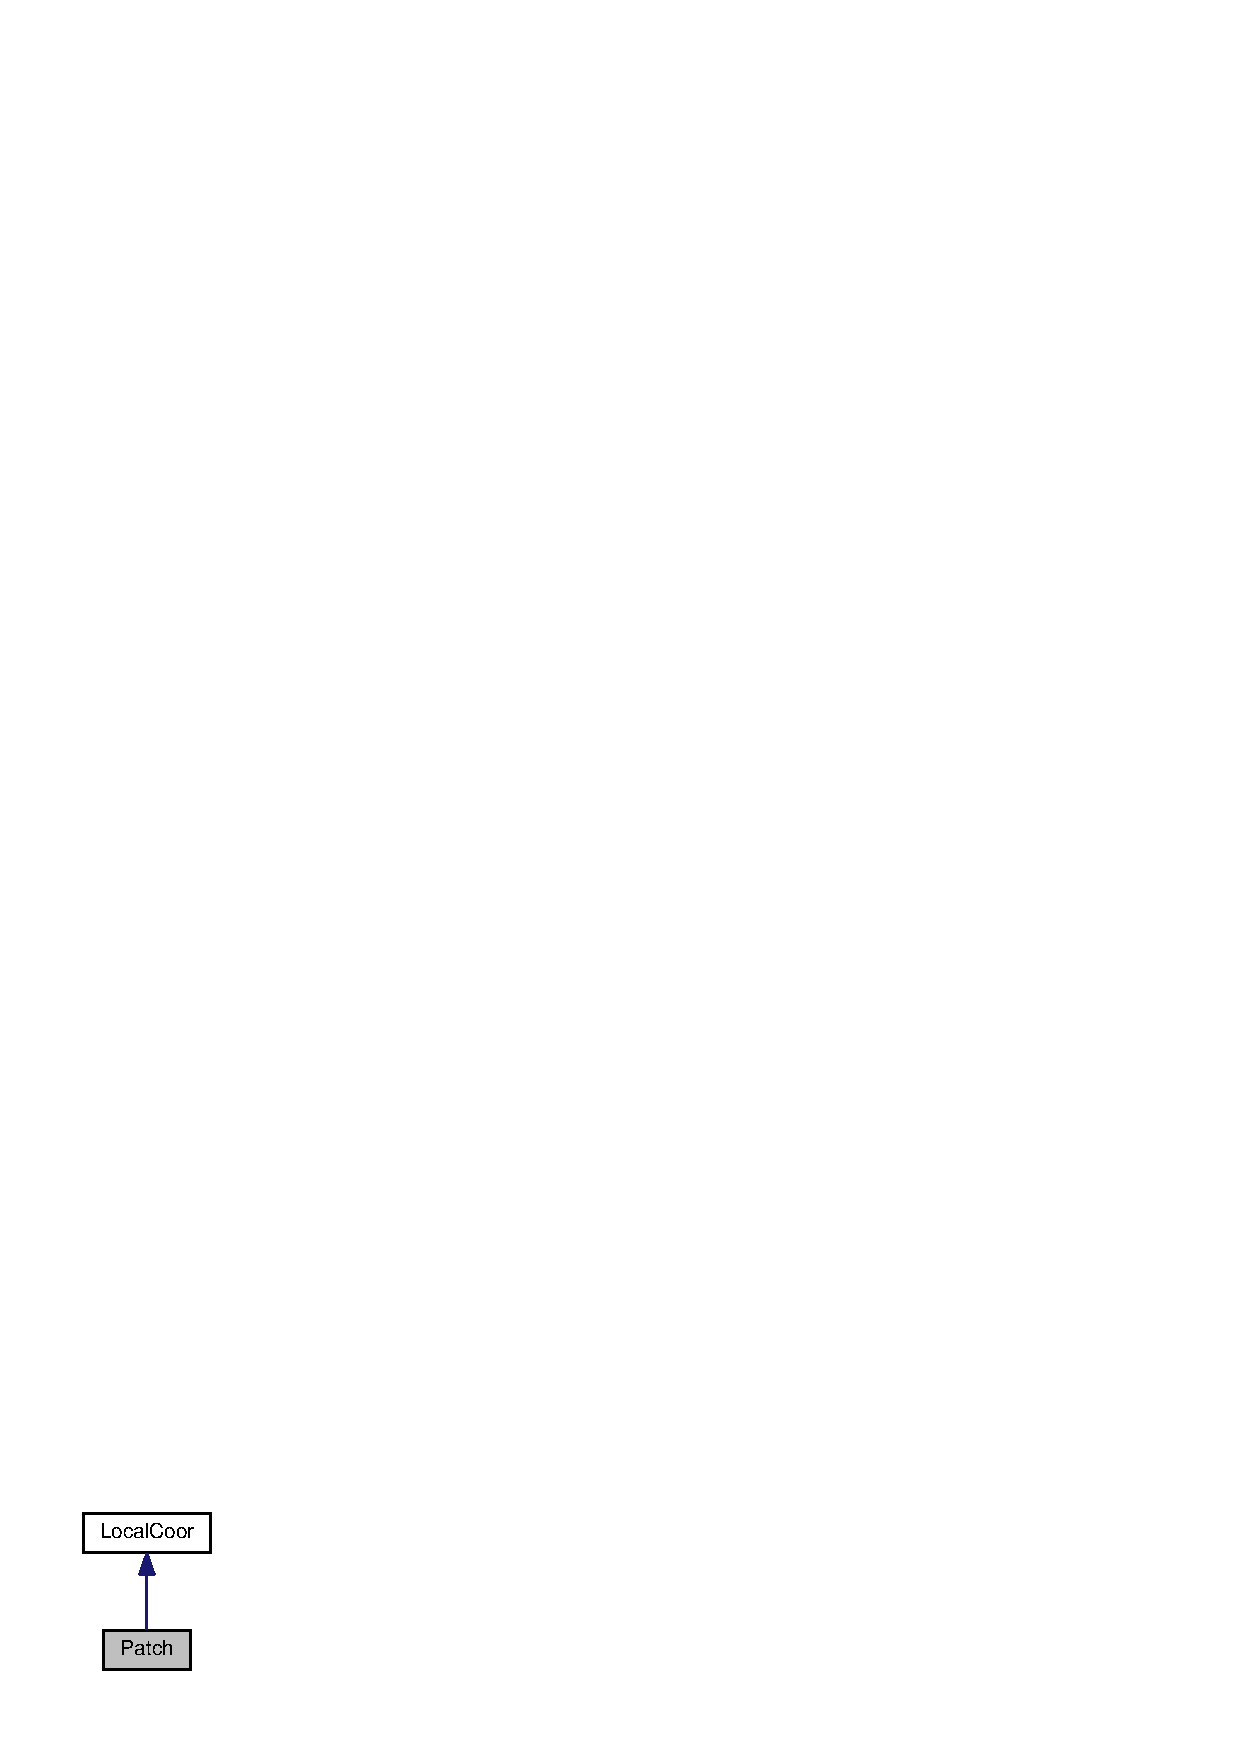
\includegraphics[width=266pt]{classPatch__inherit__graph}
\end{center}
\end{figure}


Collaboration diagram for Patch\+:\nopagebreak
\begin{figure}[H]
\begin{center}
\leavevmode
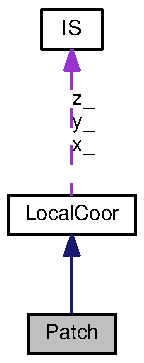
\includegraphics[width=266pt]{classPatch__coll__graph}
\end{center}
\end{figure}
\subsection*{Public Member Functions}
\begin{DoxyCompactItemize}
\item 
\hypertarget{classPatch_a74d349d49bdf800d6f7d6c31c7f39eb3}{{\bfseries Patch} (Patch\+\_\+\+Group\+\_\+s group, std\+::string name, int normal, multivec$<$ 2, size\+\_\+t $>$ indices, std\+::vector$<$ array$<$ real, 1 $>$ $>$ x, std\+::vector$<$ array$<$ size\+\_\+t, 1 $>$ $>$ nx, patch\+\_\+v\+\_\+bou\+\_\+type v\+\_\+bou)}\label{classPatch_a74d349d49bdf800d6f7d6c31c7f39eb3}

\item 
\hypertarget{classPatch_af0311eccfd4f4fd356785f7b23dc8fa2}{void {\bfseries set\+\_\+v\+\_\+bou} (std\+::string equ\+\_\+name, std\+::vector$<$ array$<$ real, 1 $>$ $>$ v\+\_\+bou)}\label{classPatch_af0311eccfd4f4fd356785f7b23dc8fa2}

\item 
\hypertarget{classPatch_a2af23d9c0ebbb60d35c24bb3fb582b64}{void {\bfseries create\+\_\+faces} ()}\label{classPatch_a2af23d9c0ebbb60d35c24bb3fb582b64}

\item 
\hypertarget{classPatch_ae57b4223cce6c1ed9dbaaa5080a2501a}{void {\bfseries grid\+\_\+nbrs} ()}\label{classPatch_ae57b4223cce6c1ed9dbaaa5080a2501a}

\item 
\hypertarget{classPatch_ae91999227e29d49f6f762b18e03fb5ac}{void {\bfseries write\+\_\+binary} (std\+::string equ\+\_\+name)}\label{classPatch_ae91999227e29d49f6f762b18e03fb5ac}

\end{DoxyCompactItemize}
\begin{Indent}{\bf value inspection and manipulation}\par
\begin{DoxyCompactItemize}
\item 
\hypertarget{classPatch_a08dda4968df785bc8a781eeed5132826}{real {\bfseries min} (std\+::string const \&equ\+\_\+name) const }\label{classPatch_a08dda4968df785bc8a781eeed5132826}

\item 
\hypertarget{classPatch_a8c5d72cafac1cb85958bd4190001ebd3}{real {\bfseries max} (std\+::string const \&equ\+\_\+name) const }\label{classPatch_a8c5d72cafac1cb85958bd4190001ebd3}

\end{DoxyCompactItemize}
\end{Indent}
\subsection*{Public Attributes}
\begin{DoxyCompactItemize}
\item 
\hypertarget{classPatch_a93fff2891647c4109c16cb4ec2079545}{Patch\+\_\+\+Group\+\_\+w {\bfseries group\+\_\+}}\label{classPatch_a93fff2891647c4109c16cb4ec2079545}

\item 
\hypertarget{classPatch_a133d268d88897aef8b20ca7da98b9cdb}{std\+::string {\bfseries name\+\_\+}}\label{classPatch_a133d268d88897aef8b20ca7da98b9cdb}

\item 
\hypertarget{classPatch_a01951c7c7aec32d184e11869ab23877d}{int {\bfseries normal\+\_\+}}\label{classPatch_a01951c7c7aec32d184e11869ab23877d}

\item 
\hypertarget{classPatch_a3beca2ce16697d8e8097ba92ee6bdc29}{coor\+\_\+type {\bfseries coor\+\_\+}}\label{classPatch_a3beca2ce16697d8e8097ba92ee6bdc29}

\item 
\hypertarget{classPatch_aa69a7e422610ce91ad4fb60c88cadbf0}{cell\+\_\+count\+\_\+type {\bfseries nx\+\_\+}}\label{classPatch_aa69a7e422610ce91ad4fb60c88cadbf0}

\item 
\hypertarget{classPatch_aea44744ce3a7d51831f67014bc89867d}{patch\+\_\+v\+\_\+bou\+\_\+type {\bfseries v\+\_\+bou\+\_\+}}\label{classPatch_aea44744ce3a7d51831f67014bc89867d}

\item 
\hypertarget{classPatch_af272c0110d640ddd191492fc9cc62990}{multivec$<$ 2, size\+\_\+t $>$ {\bfseries indices\+\_\+}}\label{classPatch_af272c0110d640ddd191492fc9cc62990}

\item 
\hypertarget{classPatch_aaa96294c5c204449ca53209b040ae06c}{array$<$ size\+\_\+t, 1 $>$ {\bfseries npatch\+\_\+}}\label{classPatch_aaa96294c5c204449ca53209b040ae06c}

\item 
\hypertarget{classPatch_a6d0bbabb9b7b1928bda12255b312fedd}{array$<$ Face\+\_\+s, 2 $>$ {\bfseries faces\+\_\+}}\label{classPatch_a6d0bbabb9b7b1928bda12255b312fedd}

\end{DoxyCompactItemize}


The documentation for this class was generated from the following files\+:\begin{DoxyCompactItemize}
\item 
/nfs/stak/students/r/rymalc/\+Documents/\+Programming/\+C++/\+Diffusion2\+D/include/\+Diff2\+D/patch.\+hpp\item 
/nfs/stak/students/r/rymalc/\+Documents/\+Programming/\+C++/\+Diffusion2\+D/src/\+Diff2\+D/patch.\+cpp\end{DoxyCompactItemize}

\hypertarget{classPatch__Group}{
\section{Patch\_\-Group Class Reference}
\label{classPatch__Group}\index{Patch\_\-Group@{Patch\_\-Group}}
}
\subsection*{Public Member Functions}
\begin{DoxyCompactItemize}
\item 
\hypertarget{classPatch__Group_aca3d4f7109706b6db9b0c928649c87a4}{
{\bfseries Patch\_\-Group} (Prob\_\-s prob, std::string name, std::map$<$ std::string, real $>$ v\_\-0, std::map$<$ std::string, real $>$ S, real v\_\-0\_\-point\mbox{[}2\mbox{]})}
\label{classPatch__Group_aca3d4f7109706b6db9b0c928649c87a4}

\item 
\hypertarget{classPatch__Group_abb0f6e18c5833efbe20634c1e4aabe9b}{
Patch\_\-s {\bfseries create\_\-patch} (std::string name, int normal, std::vector$<$ size\_\-t $>$ indicesx, std::vector$<$ size\_\-t $>$ indicesy, std::vector$<$ size\_\-t $>$ indicesz, patch\_\-v\_\-bou\_\-type v\_\-bou)}
\label{classPatch__Group_abb0f6e18c5833efbe20634c1e4aabe9b}

\item 
\hypertarget{classPatch__Group_ada9f56e3be9279ff5d555f2192cfc45b}{
real {\bfseries reset\_\-s} (std::string equ\_\-name)}
\label{classPatch__Group_ada9f56e3be9279ff5d555f2192cfc45b}

\item 
\hypertarget{classPatch__Group_a326628f83583bb2194f8c82548e9b6b3}{
std::vector$<$ Face\_\-s $>$ {\bfseries faces} ()}
\label{classPatch__Group_a326628f83583bb2194f8c82548e9b6b3}

\item 
\hypertarget{classPatch__Group_a3de7d3df9923795d4cbfa4d908e53598}{
void {\bfseries write} (std::string equ\_\-name, std::ofstream \&ofs)}
\label{classPatch__Group_a3de7d3df9923795d4cbfa4d908e53598}

\end{DoxyCompactItemize}
\subsection*{Public Attributes}
\begin{DoxyCompactItemize}
\item 
\hypertarget{classPatch__Group_a637b27a0562076f78bf9b0698ac3609e}{
std::vector$<$ Patch\_\-s $>$ {\bfseries patches\_\-}}
\label{classPatch__Group_a637b27a0562076f78bf9b0698ac3609e}

\item 
\hypertarget{classPatch__Group_ac8d91a179d394f1d3d355d82ceb2dd2e}{
Prob\_\-w {\bfseries prob\_\-}}
\label{classPatch__Group_ac8d91a179d394f1d3d355d82ceb2dd2e}

\item 
\hypertarget{classPatch__Group_ac28afa5068ea65b91ce4d708f63c5a3a}{
std::string {\bfseries name\_\-}}
\label{classPatch__Group_ac28afa5068ea65b91ce4d708f63c5a3a}

\item 
\hypertarget{classPatch__Group_ae080e43ddd30ced473794b12a1cb3ccf}{
std::map$<$ std::string, real $>$ {\bfseries v\_\-0\_\-}}
\label{classPatch__Group_ae080e43ddd30ced473794b12a1cb3ccf}

\item 
\hypertarget{classPatch__Group_aaad946bd88382b1e2e30cd1278632ace}{
std::map$<$ std::string, real $>$ {\bfseries S\_\-}}
\label{classPatch__Group_aaad946bd88382b1e2e30cd1278632ace}

\item 
\hypertarget{classPatch__Group_aec0690749d93e67521293acb28c81fb1}{
real {\bfseries v\_\-0\_\-point\_\-} \mbox{[}2\mbox{]}}
\label{classPatch__Group_aec0690749d93e67521293acb28c81fb1}

\end{DoxyCompactItemize}


The documentation for this class was generated from the following files:\begin{DoxyCompactItemize}
\item 
/nfs/stak/students/r/rymalc/Documents/Programming/C++/Diffusion2D/include/Diff2D/patch\_\-group.hpp\item 
/nfs/stak/students/r/rymalc/Documents/Programming/C++/Diffusion2D/src/Diff2D/patch\_\-group.cpp\end{DoxyCompactItemize}

\hypertarget{structpoint}{\section{point Struct Reference}
\label{structpoint}\index{point@{point}}
}
\subsection*{Public Member Functions}
\begin{DoxyCompactItemize}
\item 
\hypertarget{structpoint_a08bc9dbc1d0c3e660da63517b81b6bfc}{{\bfseries point} (real nx, real ny, real nz)}\label{structpoint_a08bc9dbc1d0c3e660da63517b81b6bfc}

\item 
\hypertarget{structpoint_ad8f9091344c2c79e6489d088af9e8728}{{\bfseries point} (\hyperlink{structpoint}{point} const \&p)}\label{structpoint_ad8f9091344c2c79e6489d088af9e8728}

\item 
\hypertarget{structpoint_a1c0d75148e183e0fd2a98600f4874146}{real \& {\bfseries operator\mbox{[}$\,$\mbox{]}} (unsigned int i)}\label{structpoint_a1c0d75148e183e0fd2a98600f4874146}

\end{DoxyCompactItemize}
\subsection*{Public Attributes}
\begin{DoxyCompactItemize}
\item 
\hypertarget{structpoint_a86514a6ef1f39599395ca289eca1aec2}{\begin{tabbing}
xx\=xx\=xx\=xx\=xx\=xx\=xx\=xx\=xx\=\kill
union \{\\
\hypertarget{unionpoint_1_1@1_addef4776bcfa7b51f06e55d76cc93cf9}{\>struct \{\\
\hypertarget{structpoint_1_1@1_1_1@3_a09a1cd2a5685e11a1afe789034b1e7ce}{\>\>real {\bfseries x}\\
\hypertarget{structpoint_1_1@1_1_1@3_af0aeda495b0d365bb5cda1c50c469dbc}{\>\>real {\bfseries y}\\
\hypertarget{structpoint_1_1@1_1_1@3_ad7b4a1d203a98754340ce3e7ea9ab686}{\>\>real {\bfseries z}\\
\>\} }\label{unionpoint_1_1@1_addef4776bcfa7b51f06e55d76cc93cf9}
\\
\hypertarget{unionpoint_1_1@1_af90ee4c5355cf7c936be57154fc3f002}{\>real {\bfseries v} \mbox{[}3\mbox{]}\\
\}; }\label{structpoint_a86514a6ef1f39599395ca289eca1aec2}
\\

\end{tabbing}\end{DoxyCompactItemize}


The documentation for this struct was generated from the following file\+:\begin{DoxyCompactItemize}
\item 
/nfs/stak/students/r/rymalc/\+Documents/\+Programming/\+C++/\+Diffusion2\+D/include/\+Diff2\+D/point.\+hpp\end{DoxyCompactItemize}

\hypertarget{classpoint__not__found}{
\section{point\_\-not\_\-found Class Reference}
\label{classpoint__not__found}\index{point\_\-not\_\-found@{point\_\-not\_\-found}}
}


The documentation for this class was generated from the following file:\begin{DoxyCompactItemize}
\item 
/nfs/stak/students/r/rymalc/Documents/Programming/C++/Diffusion2D/include/Diff2D/equation.hpp\end{DoxyCompactItemize}

\hypertarget{classProb}{\section{Prob Class Reference}
\label{classProb}\index{Prob@{Prob}}
}


Problem  




{\ttfamily \#include $<$prob.\+hpp$>$}



Inheritance diagram for Prob\+:\nopagebreak
\begin{figure}[H]
\begin{center}
\leavevmode
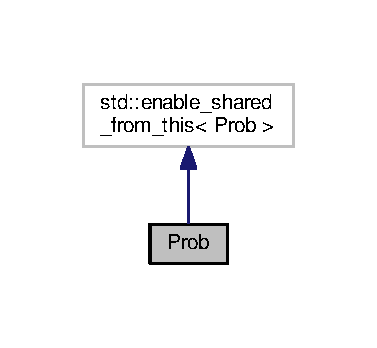
\includegraphics[width=181pt]{classProb__inherit__graph}
\end{center}
\end{figure}


Collaboration diagram for Prob\+:\nopagebreak
\begin{figure}[H]
\begin{center}
\leavevmode
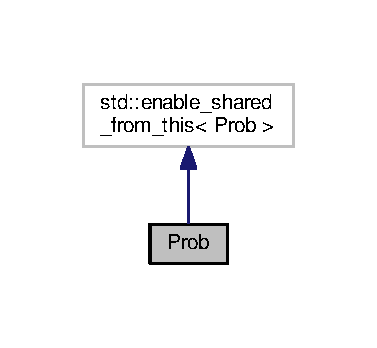
\includegraphics[width=181pt]{classProb__coll__graph}
\end{center}
\end{figure}
\subsection*{Public Member Functions}
\begin{DoxyCompactItemize}
\item 
\hypertarget{classProb_a4d146873812b11594835eeb221057ce3}{{\bfseries Prob} (std\+::string name, coor\+\_\+type x, cell\+\_\+count\+\_\+type nx, int it\+\_\+max\+\_\+1, int it\+\_\+max\+\_\+2)}\label{classProb_a4d146873812b11594835eeb221057ce3}

\item 
\hypertarget{classProb_a9e42af858cc616a84ffa860ed30703cc}{Equation\+\_\+\+Prob\+\_\+s {\bfseries create\+\_\+equation} (std\+::string name, real k, real alpha, real alpha\+\_\+source)}\label{classProb_a9e42af858cc616a84ffa860ed30703cc}

\item 
\hypertarget{classProb_abb05f9a8629633d7509ec035128c3012}{Patch\+\_\+\+Group\+\_\+s {\bfseries create\+\_\+patch\+\_\+group} (std\+::string name, std\+::map$<$ std\+::string, real $>$ v\+\_\+0, std\+::map$<$ std\+::string, real $>$ S, \hyperlink{structpoint}{point} v\+\_\+0\+\_\+point)}\label{classProb_abb05f9a8629633d7509ec035128c3012}

\item 
\hypertarget{classProb_a30084f3c079cf517bdffdad065eee5dc}{std\+::vector$<$ Face\+\_\+s $>$ {\bfseries faces} () const }\label{classProb_a30084f3c079cf517bdffdad065eee5dc}

\item 
int \hyperlink{classProb_ad4de9e5a4bf13c03e2ba243b884b75d7}{solve} (std\+::string name, real cond, size\+\_\+t it\+\_\+outer, real R\+\_\+outer)
\begin{DoxyCompactList}\small\item\em solve \end{DoxyCompactList}\item 
int \hyperlink{classProb_ad16bc67a7a966dd5b6ba38afbe85a860}{solve\+\_\+serial} (std\+::string name, real cond, size\+\_\+t it\+\_\+outer, real R\+\_\+outer)
\item 
int \hyperlink{classProb_a3d2e422acfd8bf712d7fca87c5bc04ca}{solve2} (std\+::string equ\+\_\+name, real cond\+\_\+outer, real inner\+\_\+out\+\_\+ratio)
\begin{DoxyCompactList}\small\item\em solve2 \end{DoxyCompactList}\item 
\hypertarget{classProb_a187e846a4f4eed21758efaa63ede9ec1}{void {\bfseries save} ()}\label{classProb_a187e846a4f4eed21758efaa63ede9ec1}

\item 
\hypertarget{classProb_ad790058d97221b21c665d550650c15ad}{void {\bfseries write} (std\+::string equ\+\_\+name)}\label{classProb_ad790058d97221b21c665d550650c15ad}

\item 
\hypertarget{classProb_a06e9e4b07d84c253b313b6d490776353}{void {\bfseries write\+\_\+binary} (std\+::string equ\+\_\+name)}\label{classProb_a06e9e4b07d84c253b313b6d490776353}

\end{DoxyCompactItemize}
\begin{Indent}{\bf value inspection and manipulation}\par
\begin{DoxyCompactItemize}
\item 
\hypertarget{classProb_a070c8fd90e9380ce16bcbd71843dee87}{real {\bfseries max} (std\+::string const \&equ\+\_\+name) const }\label{classProb_a070c8fd90e9380ce16bcbd71843dee87}

\item 
\hypertarget{classProb_a7cd3cf3838b2f434db946420dddef4c3}{real {\bfseries min} (std\+::string const \&equ\+\_\+name) const }\label{classProb_a7cd3cf3838b2f434db946420dddef4c3}

\item 
\hypertarget{classProb_a081a8b2a0890f3756e77d2b641910a84}{real {\bfseries grad\+\_\+max} (std\+::string const \&equ\+\_\+name) const }\label{classProb_a081a8b2a0890f3756e77d2b641910a84}

\item 
\hypertarget{classProb_ad19b211a5a372a8f43e56897bf7ca9d3}{real {\bfseries grad\+\_\+min} (std\+::string const \&equ\+\_\+name) const }\label{classProb_ad19b211a5a372a8f43e56897bf7ca9d3}

\item 
\hypertarget{classProb_ae640aa1c7afdc30de6b49b576673c4cc}{void {\bfseries value\+\_\+add} (std\+::string const \&equ\+\_\+name, real const \&v)}\label{classProb_ae640aa1c7afdc30de6b49b576673c4cc}

\item 
\hypertarget{classProb_ace52b307acd315c5243f3aa676f2d550}{void {\bfseries value\+\_\+add} (std\+::string const \&equ\+\_\+name, array$<$ real, 2 $>$ const \&v)}\label{classProb_ace52b307acd315c5243f3aa676f2d550}

\item 
\hypertarget{classProb_a12688abbc76b07d448b2ed25d0b439a6}{void {\bfseries value\+\_\+normalize} (std\+::string const \&equ\+\_\+name)}\label{classProb_a12688abbc76b07d448b2ed25d0b439a6}

\item 
\hypertarget{classProb_a4fd63fbff17359e851c4078d82b6449a}{void {\bfseries value\+\_\+clamp\+\_\+per\+\_\+group} (std\+::string const \&name, real a, real const \&b)}\label{classProb_a4fd63fbff17359e851c4078d82b6449a}

\item 
\hypertarget{classProb_a7bb25a9a766484c678d7e23e4b5ea4a7}{void {\bfseries copy\+\_\+value\+\_\+to\+\_\+source} (std\+::string equ\+\_\+name\+\_\+from, std\+::string equ\+\_\+name\+\_\+to)}\label{classProb_a7bb25a9a766484c678d7e23e4b5ea4a7}

\end{DoxyCompactItemize}
\end{Indent}
\subsection*{Public Attributes}
\begin{DoxyCompactItemize}
\item 
\hypertarget{classProb_a63da8c35707c884a7f2960b18e8b5e30}{std\+::vector$<$ Patch\+\_\+\+Group\+\_\+s $>$ {\bfseries patch\+\_\+groups\+\_\+}}\label{classProb_a63da8c35707c884a7f2960b18e8b5e30}

\item 
\hypertarget{classProb_af34172c6eced00a603e92e0cf17e4953}{std\+::string {\bfseries name\+\_\+}}\label{classProb_af34172c6eced00a603e92e0cf17e4953}

\item 
\hypertarget{classProb_ac18ce288649f196b15137b88bfe374de}{std\+::vector$<$ array$<$ real, 1 $>$ $>$ {\bfseries x\+\_\+}}\label{classProb_ac18ce288649f196b15137b88bfe374de}

\item 
\hypertarget{classProb_a59f92ce7194950bf4c89d00af62c7b51}{std\+::vector$<$ array$<$ size\+\_\+t, 1 $>$ $>$ {\bfseries nx\+\_\+}}\label{classProb_a59f92ce7194950bf4c89d00af62c7b51}

\item 
\hypertarget{classProb_ac78ec4ce0542942cbfdb62e2737b149e}{std\+::map$<$ std\+::string, \\*
Equation\+\_\+\+Prob\+\_\+s $>$ {\bfseries equs\+\_\+}}\label{classProb_ac78ec4ce0542942cbfdb62e2737b149e}

\item 
\hypertarget{classProb_a4414250c2bd8f6aa6cfc9488c3993092}{size\+\_\+t {\bfseries it\+\_\+max\+\_\+inner\+\_\+}}\label{classProb_a4414250c2bd8f6aa6cfc9488c3993092}

\item 
\hypertarget{classProb_aa52011388c8c265ffc71c010a4b61f8f}{size\+\_\+t {\bfseries it\+\_\+max\+\_\+outer\+\_\+}}\label{classProb_aa52011388c8c265ffc71c010a4b61f8f}

\end{DoxyCompactItemize}


\subsection{Detailed Description}
Problem 

\subsection{Member Function Documentation}
\hypertarget{classProb_ad4de9e5a4bf13c03e2ba243b884b75d7}{\index{Prob@{Prob}!solve@{solve}}
\index{solve@{solve}!Prob@{Prob}}
\subsubsection[{solve}]{\setlength{\rightskip}{0pt plus 5cm}int Prob\+::solve (
\begin{DoxyParamCaption}
\item[{std\+::string}]{name, }
\item[{real}]{cond, }
\item[{size\+\_\+t}]{it\+\_\+outer, }
\item[{real}]{R\+\_\+outer}
\end{DoxyParamCaption}
)}}\label{classProb_ad4de9e5a4bf13c03e2ba243b884b75d7}


solve 


\begin{DoxyParams}{Parameters}
{\em name} & name of variable to solve \\
\hline
{\em cond} & residual stop condition \\
\hline
{\em it\+\_\+outer} & current iteration of outer loop for purpose of displaying \\
\hline
{\em R\+\_\+outer} & current residual of outer loop for purpose of displaying \\
\hline
\end{DoxyParams}
\hypertarget{classProb_a3d2e422acfd8bf712d7fca87c5bc04ca}{\index{Prob@{Prob}!solve2@{solve2}}
\index{solve2@{solve2}!Prob@{Prob}}
\subsubsection[{solve2}]{\setlength{\rightskip}{0pt plus 5cm}int Prob\+::solve2 (
\begin{DoxyParamCaption}
\item[{std\+::string}]{equ\+\_\+name, }
\item[{real}]{cond\+\_\+outer, }
\item[{real}]{inner\+\_\+out\+\_\+ratio}
\end{DoxyParamCaption}
)}}\label{classProb_a3d2e422acfd8bf712d7fca87c5bc04ca}


solve2 


\begin{DoxyParams}{Parameters}
{\em equ\+\_\+name} & name \\
\hline
{\em cond\+\_\+outer} & residual stop condition of outer loop \\
\hline
{\em inner\+\_\+outer\+\_\+ratio} & ratio of inner loop residual stop condition to current outer loop residual \\
\hline
{\em ver} & verbosity \\
\hline
\end{DoxyParams}
\hypertarget{classProb_ad16bc67a7a966dd5b6ba38afbe85a860}{\index{Prob@{Prob}!solve\+\_\+serial@{solve\+\_\+serial}}
\index{solve\+\_\+serial@{solve\+\_\+serial}!Prob@{Prob}}
\subsubsection[{solve\+\_\+serial}]{\setlength{\rightskip}{0pt plus 5cm}int Prob\+::solve\+\_\+serial (
\begin{DoxyParamCaption}
\item[{std\+::string}]{name, }
\item[{real}]{cond, }
\item[{size\+\_\+t}]{it\+\_\+outer, }
\item[{real}]{R\+\_\+outer}
\end{DoxyParamCaption}
)}}\label{classProb_ad16bc67a7a966dd5b6ba38afbe85a860}
\begin{DoxyRefDesc}{Todo}
\item[\hyperlink{todo__todo000001}{Todo}]move this to class variable to avoid excess alloc! \end{DoxyRefDesc}


The documentation for this class was generated from the following files\+:\begin{DoxyCompactItemize}
\item 
/nfs/stak/students/r/rymalc/\+Documents/\+Programming/\+C++/\+Diffusion2\+D/include/\+Diff2\+D/prob.\+hpp\item 
/nfs/stak/students/r/rymalc/\+Documents/\+Programming/\+C++/\+Diffusion2\+D/src/\+Diff2\+D/prob.\+cpp\end{DoxyCompactItemize}

\hypertarget{structTerm}{\section{Term Struct Reference}
\label{structTerm}\index{Term@{Term}}
}
\subsection*{Public Member Functions}
\begin{DoxyCompactItemize}
\item 
\hypertarget{structTerm_a90008c143070b0544ea0a5de0dd0d651}{real {\bfseries prod} ()}\label{structTerm_a90008c143070b0544ea0a5de0dd0d651}

\end{DoxyCompactItemize}
\subsection*{Public Attributes}
\begin{DoxyCompactItemize}
\item 
\hypertarget{structTerm_a5b8e26faad37a4317ce722efbb2fb345}{real {\bfseries a}}\label{structTerm_a5b8e26faad37a4317ce722efbb2fb345}

\item 
\hypertarget{structTerm_adc6281bf7884d8b213aa98a701b4e578}{real {\bfseries y}}\label{structTerm_adc6281bf7884d8b213aa98a701b4e578}

\end{DoxyCompactItemize}


The documentation for this struct was generated from the following file\+:\begin{DoxyCompactItemize}
\item 
/nfs/stak/students/r/rymalc/\+Documents/\+Programming/\+C++/\+Diffusion2\+D/include/\+Diff2\+D/face.\+hpp\end{DoxyCompactItemize}

\chapter{File Documentation}
\hypertarget{types_8hpp}{\section{/nfs/stak/students/r/rymalc/\+Documents/\+Programming/\+C++/\+Diffusion2\+D/include/\+Diff2\+D/types.hpp File Reference}
\label{types_8hpp}\index{/nfs/stak/students/r/rymalc/\+Documents/\+Programming/\+C++/\+Diffusion2\+D/include/\+Diff2\+D/types.\+hpp@{/nfs/stak/students/r/rymalc/\+Documents/\+Programming/\+C++/\+Diffusion2\+D/include/\+Diff2\+D/types.\+hpp}}
}
{\ttfamily \#include $<$map$>$}\\*
{\ttfamily \#include $<$math-\/array/array.\+hpp$>$}\\*
Include dependency graph for types.\+hpp\+:\nopagebreak
\begin{figure}[H]
\begin{center}
\leavevmode
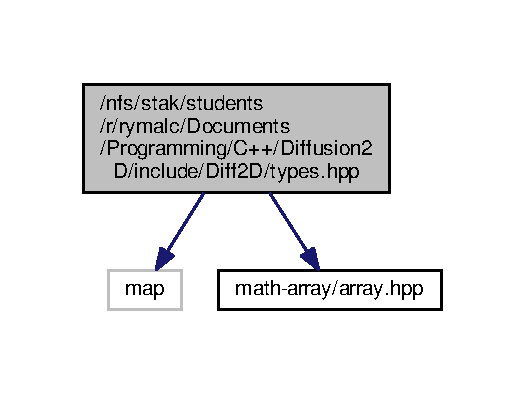
\includegraphics[width=252pt]{types_8hpp__incl}
\end{center}
\end{figure}
This graph shows which files directly or indirectly include this file\+:
\nopagebreak
\begin{figure}[H]
\begin{center}
\leavevmode
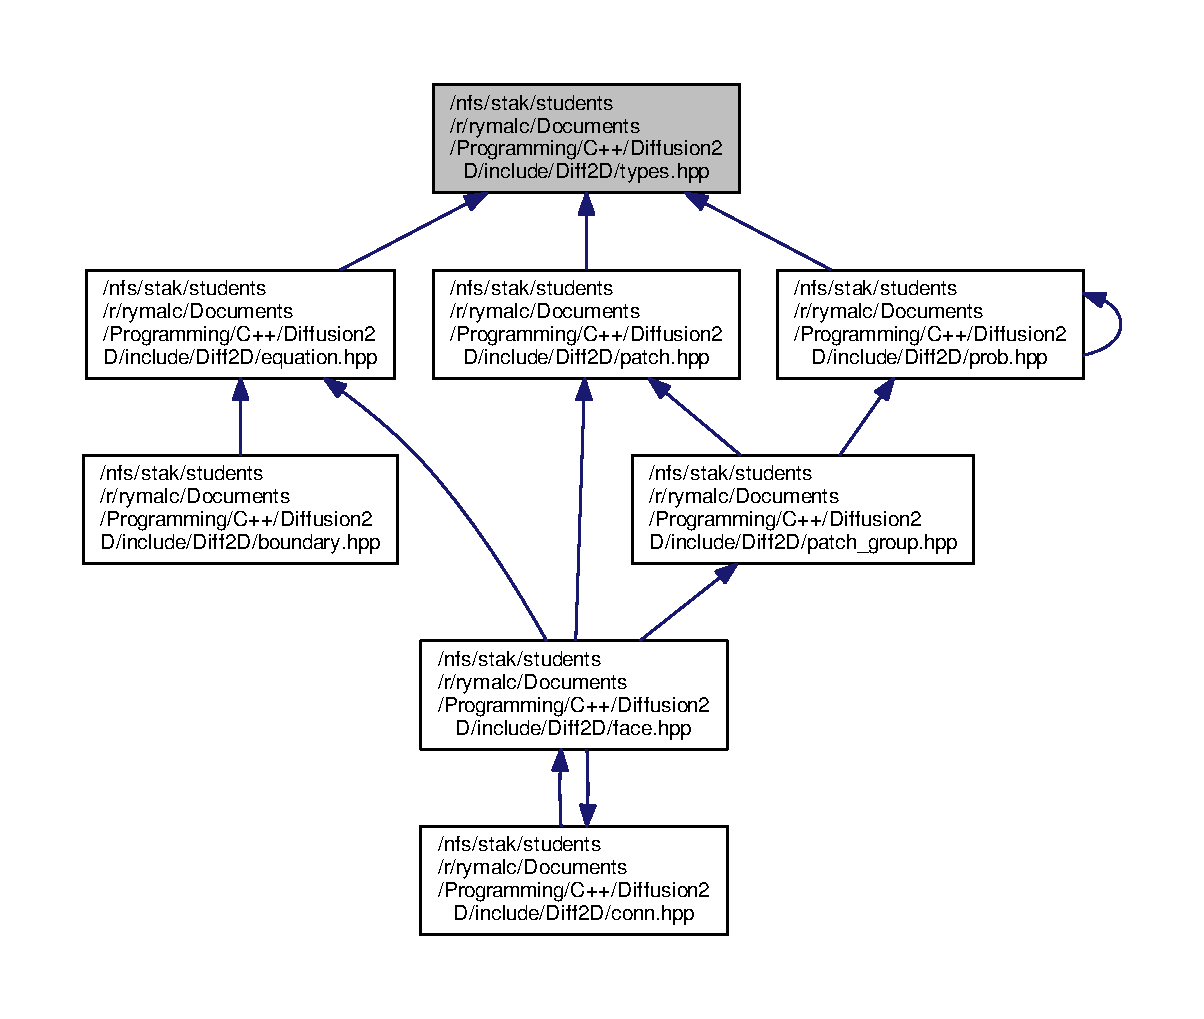
\includegraphics[width=350pt]{types_8hpp__dep__incl}
\end{center}
\end{figure}
\subsection*{Typedefs}
\begin{DoxyCompactItemize}
\item 
\hypertarget{types_8hpp_a72b5116b97ac88f6fc3857e258722059}{typedef std\+::vector$<$ array\\*
$<$ real, 1 $>$ $>$ {\bfseries coor\+\_\+type}}\label{types_8hpp_a72b5116b97ac88f6fc3857e258722059}

\item 
\hypertarget{types_8hpp_a6be640374a9e488d66b17b9620cf3530}{typedef std\+::vector$<$ array\\*
$<$ size\+\_\+t, 1 $>$ $>$ {\bfseries cell\+\_\+count\+\_\+type}}\label{types_8hpp_a6be640374a9e488d66b17b9620cf3530}

\item 
\hypertarget{types_8hpp_abc8ea65a7638279dbdeb08986cc52356}{typedef std\+::vector\\*
$<$ std\+::shared\+\_\+ptr$<$ \hyperlink{structboundary}{boundary} $>$ $>$ {\bfseries patch\+\_\+v\+\_\+bou\+\_\+edge\+\_\+vec\+\_\+type}}\label{types_8hpp_abc8ea65a7638279dbdeb08986cc52356}

\item 
\hypertarget{types_8hpp_a2fa707ce7e576fce891e514ffb845e0e}{typedef multivec\\*
$<$ 2, std\+::shared\+\_\+ptr$<$ \hyperlink{structboundary}{boundary} $>$ $>$ {\bfseries equ\+\_\+v\+\_\+bou\+\_\+type}}\label{types_8hpp_a2fa707ce7e576fce891e514ffb845e0e}

\item 
\hypertarget{types_8hpp_a69c2d12322d22dabdf890609b4435f0f}{typedef multivec\\*
$<$ 3, std\+::shared\+\_\+ptr$<$ \hyperlink{structboundary}{boundary} $>$ $>$ {\bfseries patch\+\_\+v\+\_\+bou\+\_\+vec\+\_\+type}}\label{types_8hpp_a69c2d12322d22dabdf890609b4435f0f}

\item 
\hypertarget{types_8hpp_a07d5bcc029b5ac042dfd7b3c967f51a9}{typedef std\+::map$<$ std\+::string, \\*
patch\+\_\+v\+\_\+bou\+\_\+vec\+\_\+type $>$ {\bfseries patch\+\_\+v\+\_\+bou\+\_\+type}}\label{types_8hpp_a07d5bcc029b5ac042dfd7b3c967f51a9}

\end{DoxyCompactItemize}

%--- End generated contents ---

% Index
\newpage
\phantomsection
\addcontentsline{toc}{chapter}{Index}
\printindex

\end{document}
